\documentclass[msc,numbers,fleqn]{coppe} %% Mestrado: "msc"; Doutorado: "dsc";
\usepackage{amsmath,amssymb}
\usepackage[hidelinks]{hyperref}
\usepackage{xcolor}
\usepackage{float}
\usepackage{indentfirst}
\usepackage{tabularx}
\usepackage{graphicx}


\setlength{\mathindent}{0pt}

\makelosymbols
\makeloabbreviations

\begin{document}
  \title{Análise de longo prazo de membranas comerciais no tratamento de água de produção via destilação por membranas}
  \foreigntitle{Temporal analysis of commercial membranes in the treatment of produced water via membrane distillation.}
  \author{Antonio Victor}{de Souza Correa}
  \advisor{Prof.}{Carolina}{Palma Naveira Cotta}{D.Sc.}
  %\advisor{Prof.}{Nome do Segundo Orientador}{Sobrenome}{Ph.D.}
  %\advisor{Prof.}{Nome do Terceiro Orientador}{Sobrenome}{D.Sc.}

  %\examiner{Prof.}{Nome do Primeiro Examinador Sobrenome}{D.Sc.}
  %\examiner{Prof.}{Nome do Segundo Examinador Sobrenome}{Ph.D.}
  %\examiner{Prof.}{Nome do Terceiro Examinador Sobrenome}{D.Sc.}
  %\examiner{Prof.}{Nome do Quarto Examinador Sobrenome}{Ph.D.}
  %\examiner{Prof.}{Nome do Quinto Examinador Sobrenome}{Ph.D.}
  \department{PEM} %% Mudar para sigla do seu departamento
  \date{05}{2026}

  \keyword{Primeira palavra-chave}
  \keyword{Segunda palavra-chave}
  \keyword{Terceira palavra-chave}

  \maketitle

  \renewcommand{\makecatalog}{}
  \makeatletter
  \renewcommand{\makefrontpage}{}
  \renewcommand{\makecatalog}{}
  \makeatother
  \frontmatter
  %\dedication{A algu\'em cujo valor \'e digno desta dedicat\'oria.}

  %\include{Chapters/000AcknowledgmentAndAbstract/00Acknowledgment}
  \makeatletter
\renewcommand{\abstract@toptext}{
\noindent Proposta de Dissertação de Mestrado apresentada à COPPE/UFRJ como parte dos requisitos necessários para a obtenção do título de Mestre em Engenharia Mecânica.
}
\makeatother
\begin{abstract}

%A destilação por membranas aplicada ao tratamento de água de produção apresenta-se como uma tecnologia promissora para recuperação de água em processos da indústria do petróleo, devido à sua elevada rejeição de sais e capacidade de operar com soluções de alta salinidade. Entretanto, a ocorrência de mecanismos de falha, como molhamento (wetting) e incrustação (fouling), compromete a estabilidade operacional do processo ao longo do tempo, tornando necessária a avaliação do desempenho temporal das membranas empregadas. Nesse contexto, este trabalho propõe a análise experimental de membranas comerciais submetidas ao tratamento de água de produção por destilação por membranas com espaçamento de ar (AGMD), visando identificar a influência das propriedades morfológicas e operacionais na estabilidade do fluxo de permeado e na qualidade da água produzida. Para isso, serão avaliadas membranas fabricadas com diferentes materiais e suportes, previamente caracterizadas por porosimetria de fluxo capilar, microscopia digital e medições de ângulo de contato, permitindo determinar parâmetros como distribuição de poros, porosidade e pressão de entrada do líquido (LEP). Os experimentos serão conduzidos em uma bancada laboratorial instrumentada, operando com água de produção real oriunda de um campo petrolífero brasileiro, considerando condições controladas de temperatura, vazão e salinidade durante ensaios de longa duração. Além disso, pretende-se correlacionar os mecanismos de degradação observados com as características físico-químicas da água de produção e os parâmetros operacionais do processo, contribuindo para o desenvolvimento de sistemas de destilação por membranas mais confiáveis e adequados para aplicações industriais.
  

A água de produção é o principal resíduo gerado na exploração e produção de petróleo, sendo composta por água de formação, água de injeção e compostos oriundos do reservatório. Sua composição pode incluir sais dissolvidos, hidrocarbonetos, sólidos suspensos, metais e produtos químicos utilizados no processo produtivo. As características desse resíduo variam conforme a localização do campo petrolífero, as condições geológicas do reservatório e o estágio de produção do poço, tornando seu tratamento um desafio ambiental e operacional. Neste contexto, a presente dissertação tem como objetivo avaliar o desempenho de longo prazo de membranas comerciais no tratamento de água de produção via destilação por membranas, utilizando a configuração AGMD. O estudo busca investigar a influência das características morfológicas das membranas sobre o desempenho operacional e a resistência ao molhamento. As etapas já desenvolvidas incluíram a caracterização das membranas comerciais, abrangendo distribuição e diâmetro médio de poros, ângulo de contato e LEP. Também foi realizada a caracterização da água de produção utilizada nos ensaios, determinando as concentrações dos contaminantes, além de experimentos de curto prazo para avaliação preliminar do fluxo de permeado, estabilidade operacional e suscetibilidade ao molhamento das membranas. Os experimentos de longo prazo serão conduzidos com monitoramento contínuo de fluxo de permeado, condutividade, pressão e temperatura. A partir desses ensaios, serão avaliadas a estabilidade operacional das membranas, a ocorrência de molhamento e a degradação de desempenho ao longo do tempo, buscando correlacionar as propriedades morfológicas das membranas com seu comportamento operacional em aplicações prolongadas.

\end{abstract}

%\makeatletter
%\renewcommand{\foreignabstract@toptext}{
%\noindent Proposal of Master Dissertation presented to COPPE/UFRJ as a partial fulfillment of the requirements for the degree of Master in Mechanical Engineering.
%}
%\makeatother

%\begin{foreignabstract}

%Produced water is the main waste generated during oil exploration and production, consisting of formation water, injection water, and compounds originating from the reservoir. Its composition may include dissolved salts, hydrocarbons, suspended solids, metals, and chemical additives used in the production process. The characteristics of this effluent vary according to the location of the oilfield, the geological conditions of the reservoir, and the production stage of the well, making its treatment both an environmental and operational challenge. In this context, the present dissertation aims to evaluate the long-term performance of commercial membranes in the treatment of produced water via membrane distillation using the AGMD configuration. The study seeks to investigate the influence of membrane morphological characteristics on operational performance and wetting resistance. The stages already completed included the characterization of commercial membranes, encompassing pore size distribution, mean pore diameter, contact angle, and LEP. The produced water used in the experiments was also characterized by determining contaminant concentrations, in addition to conducting short-term experiments for the preliminary evaluation of permeate flux, operational stability, and membrane wetting susceptibility. Long-term experiments will be carried out with continuous monitoring of permeate flux, conductivity, pressure, and temperature. Based on these tests, membrane operational stability, wetting occurrence, and performance degradation over time will be evaluated, aiming to correlate membrane morphological properties with their operational behavior under prolonged application conditions.
  
%\end{foreignabstract}
  
  \tableofcontents
  \listoffigures
  \listoftables
  \printlosymbols
  \printloabbreviations

  \mainmatter

  \chapter{Introdu{\c c}\~ao}

%Neste capítulo são apresentadas as motivações para a realização da análise temporal de membranas comerciais no tratamento de água de produção via destilação por membranas, os objetivos do estudo e a estrutura da dissertação.

A extração de petróleo e gás natural gera como principal subproduto a água de produção, com geração estimada em aproximadamente 250 milhões de barris por dia (39,75 milhões de metros cúbicos)~\cite{w15162980, MembranePW_JSDEWES_2024}. Estima-se que, somente em 2018, a geração anual mundial de água de produção tenha atingido 6,8 bilhões de metros cúbicos, volume que tende a aumentar com o envelhecimento dos campos petrolíferos, podendo representar até 98~\% dos fluidos produzidos em poços maduros~\cite{w15234088,ALGHOUTI2019222}. 

Historicamente tratada como um rejeito da indústria petrolífera, a água de produção passou a ser reconhecida como um recurso de valor estratégico, especialmente devido ao seu potencial de reutilização em operações de reinjeção, recuperação avançada de petróleo e o aumento do rigor de regulamentações ambientais.

A água de produção é composta pela mistura entre água de formação, naturalmente presente nos reservatórios, e água de injeção, utilizada para manutenção da pressão do reservatório e mobilização do óleo residual. Sua composição varia de acordo com a geologia do reservatório e localização geográfica, podendo conter óleo disperso, sais dissolvidos, metais pesados, sólidos suspensos, compostos orgânicos e produtos químicos empregados nas operações de produção ~\cite{BEYER2020105155, ALGHOUTI2019222, w13020183}.

A crescente demanda por práticas ambientais sustentáveis e pela maximização da recuperação de hidrocarbonetos tem impulsionado o desenvolvimento de tecnologias capazes de viabilizar o reaproveitamento da água produzida. Nesse contexto, a reinjeção destaca-se como alternativa de elevada relevância técnica e econômica, uma vez que permite reduzir o consumo de água fresca, minimizar o descarte ambiental e aumentar o fator de recuperação de petróleo por meio da manutenção da pressão do reservatório e da mobilização de óleo remanescente.

Nesse contexto, o reaproveitamento da água de produção deixa de representar apenas uma alternativa para adequação ambiental, passando a desempenhar papel estratégico na indústria do petróleo. 

A reinjeção da água tratada contribui simultaneamente para atender regulamentações~\cite{OSPAR2001,EPA435,CONAMA3932007}, diminuir o consumo de água fresca e aumento do fator de recuperação de hidrocarbonetos, por meio da manutenção da pressão do reservatório e da mobilização de óleo residual. 

Entretanto, a viabilidade dessa prática está diretamente associada à qualidade da água empregada, uma vez que elevadas concentrações de óleo, sólidos suspensos e compostos incrustantes podem provocar danos ao reservatório e aos sistemas de injeção~\cite{BADER2007159, AKSTINAT2019124011}.


Diante dessa necessidade, diferentes etapas de tratamento têm sido empregadas na indústria do petróleo, abrangendo processos primários, secundários, terciários e de polimento~\cite{Amakiri2022ProducedWaterReview,Adepitan2026HybridPW,Rajbongshi2024ProducedWaterReview,Ahmadun2009PWTechnologies}. Entre as tecnologias emergentes para tratamento e reaproveitamento da água de produção, a destilação por membranas destaca-se pela elevada rejeição de sais, capacidade de operar com soluções de alta salinidade e potencial integração com fontes térmicas de baixa temperatura.

%A extração de petróleo e gás apresenta como principal subproduto a água de produção, com uma geração aproximada de 250 milhões de barris (39,75 milhões de metros cúbicos) por dia~\cite{w15162980, MembranePW_JSDEWES_2024}. Estima-se que no ano de 2018 houve uma geração anual mundial de 6,8 bilhões de metros cúbicos de água de produção, o que promove desafios econômicos e ambientais para as empresas do ramo petrolífero, uma vez que o volume de água de produção gerado aumenta com o envelhecimento do poço e pode representar até 98\% do material extraído~\cite{w15234088,ALGHOUTI2019222}. 

%Água de produção é o termo utilizado para o conjunto de águas oriundas do processo de extração, sendo composta por água de formação (água presente naturalmente nos poços de petróleo) e água de injeção (água utilizada para manutenção da pressão do poço e auxiliar na remoção do petróleo), apresentando características e contaminantes que variam em função da geologia do ponto de extração, da localização geográfica e da profundidade do poço~\cite{BEYER2020105155, ALGHOUTI2019222, w13020183}.

%Como principais constituintes da água de produção, é possível destacar óleo disperso, gases de hidrocarbonetos dissolvidos, sais inorgânicos, ácidos orgânicos, hidrocarbonetos aromáticos, cetonas, fenóis, metais pesados, materiais radioativos de ocorrência natural, partículas sólidas em suspensão, anti-incrustantes, anticorrosivos e biocidas~\cite{Ozgun, ALLEY201174}.  

%Uma vez extraída, a água de produção precisa ser tratada de acordo com sua destinação, seja para descarte ou reinjeção. Em caso de descarte, é necessário observar as regulamentações ambientais do local de extração, como a recomendação 2001/1 da convenção Oslo Paris, que determina uma concentração de 30~mg/L de óleo em água~\cite{OSPAR2001}; a agência de proteção ambiental dos Estados Unidos (USEPA) e a resolução número 393/2007 do Conselho Nacional do Meio Ambiente (CONAMA) determinam uma concentração média mensal inferior a 29~mg/L para óleos e graxas e um valor diário máximo de 42~mg/L~\cite{EPA435,CONAMA3932007}.

%Apesar das regulações impostas pelas organizações citadas anteriormente, o descarte contínuo de água de produção é um ponto de atenção, uma vez que é a principal fonte de hidrocarbonetos aromáticos policíclicos (PAHs) e petróleo em ambiente marinho, podendo ocasionar problemas agudos ou crônicos a biota marinha \cite{BEYER2020105155}. 

%No que diz respeito à água para reinjeção, a qualidade da água determina parâmetros de injeção como pressão e obstrução de poros. Nesse sentido, a análise química da água utilizada determina a dosagem adequada de anti-incrustantes e anti-corrosivos, além de atender aos requisitos recomendados de conter no máximo 10~mg/L de sólidos suspensos totais (TSS) e 42~mg/L de óleo em água. Outro ponto de atenção é a compatibilidade química entre a água a ser utilizada na reinjeção e a água de formação presente no poço, de modo a evitar reações que propiciem a precipitação de compostos inorgânicos e a formação de encrustações~\cite{BADER2007159, AKSTINAT2019124011}. 

%Mediante a necessidade de tratamento da água de produção, diferentes etapas de tratamento são empregadas para atender os requisitos das normas citadas anteriormente. De modo geral,  tais etapas de tratamento são descritas na literatura de acordo com a tecnologia empregada e o nível de contaminantes presentes, compondo quatro grupos principais: primário, secundário, terciário e polimento, de modo que a destilação por membranas pode estar presente no grupo terciário ou na etapa de polimento~\cite{Amakiri2022ProducedWaterReview,Adepitan2026HybridPW,Rajbongshi2024ProducedWaterReview,Ahmadun2009PWTechnologies}.

O processo de destilação por membrana é um processo de separação onde a força motriz é a diferença de pressão de vapor parcial decorrente da diferença de temperatura entre os dois lados da membrana. Tal membrana é hidrofóbica e microporosa, de modo a permitir apenas a passagem de vapor por meio dos poros, uma vez que a diferença de vapor parcial promove a evaporação do fluido no lado quente do módulo~\cite{Olatunji2018MDModeling,Yan2021MDWastewater,Kaur2023MDOverview,Adewole2022MDDesalination}.

O mecanismo para a recuperação do vapor varia de acordo com a geometria do módulo empregado, podendo ocorrer internamente ou externamente ao módulo. Em módulos de destilação por membrana com espaçamento de ar (AGMD) a condensação do vapor ocorre em contato com uma chapa resfriada localizada no interior do módulo, de modo que o permeado não entra em contato com o líquido de resfriamento. Nestes módulos, o espaçamento de ar é o fator mais impactante na transferência de calor e massa, uma vez que auxilia a reduzir a perda de calor por condução~\cite{Olatunji2018MDModeling,Yan2021MDWastewater,Kaur2023MDOverview,Adewole2022MDDesalination}. 

%A confiabilidade de um equipamento aplicado na industria está atrelada a capacidade de operar de acordo com os parâmetros de processo para o qual foi projetado sem apresentar falhas; A mantenabilidade de um equipamento reflete a capacidade e a facilidade da realização de reparos para restaurar a capacidade original de operação de um equipamento. Com base nesses conceitos, o conhecimento, o monitoramento e a compreensão dos modos de falha associados aos módulos de destilação por membranas tornam-se fundamentais para o adequado dimensionamento de seus componentes~\cite{smith2011}.

%Entre os possíveis modos de falha em módulos de destilação por membrana, destacam-se o molhamento (\textit{wetting}) e a incrustação (\textit{fouling}), fenômenos que exercem impacto direto na qualidade do permeado e na redução do fluxo ao longo do tempo. 

%O molhamento é um fenômeno onde o líquido a ser tratado permeia os poros da membrana hidrofóbica. Este fenômeno está ligado as propriedades morfológicas da membrana, as características do fluido e os parâmetros do processo. No que diz respeito a membrana, é possível citar o diâmetro de poro, a rugosidade e o ângulo de contato; Para o líquido, a tensão superficial e a presença de surfactantes; Para os parâmetros de processo, a velocidade do escoamento, a diferença de pressão na superfície da membrana e a temperatura~\cite{Yao2020WettabilityMD}.

%A incrustação no processo de destilação por membrana decorre de adsorção, acumulo ou precipitação na superfície da membrana. Assim como molhamento, este fenômeno é influenciado pelas propriedades da membrana, características do fluido e parâmetros do processo. A incrustação trás como principal consequência a redução da permeabilidade e consequentemente a redução do fluxo de permeado~\cite{Alkhatib2021FoulingMD}.

%Deste modo, para o correto dimensionamento e projeto de sistemas de tratamento de água de produção, é fundamental compreender o impacto dos modos de falha citados anteriormente em membranas expostas aos contaminantes presentes na água de produção por um longo período de tempo, em vista de selecionar o material adequado para compor o equipamento.

%Ante ao exposto, a presente dissertação tem como objetivo analisar os efeitos temporais em membranas comerciais durante o tratamento de água de produção via destilação por membranas, visando identificar a morfologia da membrana mais resistente às condições operacionais e avaliar a influência do tempo de operação no desempenho do processo.

Diante do exposto, a presente dissertação tem como objetivo investigar os efeitos temporais sobre membranas comerciais empregadas no tratamento de água de produção via destilação por membranas, buscando identificar as características morfológicas associadas à maior resistência às condições operacionais e avaliar a influência do tempo de operação sobre o desempenho e a estabilidade do processo. 

Para isso, realizou-se a caracterização das membranas a serem utilizadas, através de porosimetria de fluxo capilar, microscopia digital e medições de ângulo de contato. Também realizou-se a caracterização da água de produção através de métodos físico-químicos, cromatográficos e espectroscópicos para determinação dos contaminantes presentes. Por fim, serão conduzidos experiemntos de longo prazo utilizando um módulo AGMD, por um período de até trinta dias ou até a ocorrência de falhas operacionais, como molhamento ou incrustação, de modo a avaliar a estabilidade operacional e os mecanismos de degradação do processo ao longo do tempo.

%Esta dissertação é composta por este capítulo introdutório, seguida por outros cinco capítulos. O segundo capítulo abrange a revisão bibliográfica necessária para a compreensão do tema, abordando os aspectos morfológicos das membranas, as técnicas de tratamento de água de produção e os mecanismos de transferência de calor e massa presentes no processo de destilação por membranas com espaçamento de ar (AGMD). O terceiro capítulo apresenta a metodologia empregada na realização dos experimentos, a estrutura da bancada experimental e os parâmetros utilizados. O quarto capítulo apresenta e discute os resultados obtidos com os experimentos realizados. O quinto capítulo expõe as conclusões do trabalho e as considerações finais decorrentes do estudo realizado. Por fim, o sexto capítulo apresenta sugestões de trabalhos futuros.


  \chapter{Revis\~ao Bibliogr\'afica}

Visando observar o estado da arte sobre tratamento de água de produção via destilação por membranas, realizou-se o levantamento de artigos através da plataforma \emph{Scopus}, no dia 19/01/2026, utilizando as seguintes palavras-chave: "Membrane", "Distillation", "Produced Water". Também foram aplicados os seguintes filtros: período de publicação (2015 a 2025), idioma inglês, sub áreas engenharia e engenharia química, palavras chaves "Distillation" e "Produced water" e com acesso livre.

Como resultado da pesquisa, foram obtidos 537 artigos, fig.~\ref{fig:graficopublicacoes}, os quais foram avaliados com base em seus respectivos títulos e resumos, considerando pertinentes aqueles que retratam o uso de destilação por membranas para o tratamento de água de produção ou em estudos de longo prazo. Para priorizar os artigos com maior relevância, aplicou-se aos resumos o filtro "produced water", resultando em 33 artigos. De modo a observar os artigos que retratam os modos de falha do processo, também aplicaram-se os filtros "fouling", "wetting" e "swelling" ao título dos artigos, retornando 39, 24 e 1 artigo, respectivamente. Os artigos analisados até o momento são apresentados nas seções a seguir, incluindo referências citadas nos trabalhos selecionados.

\begin{figure}
    \centering
    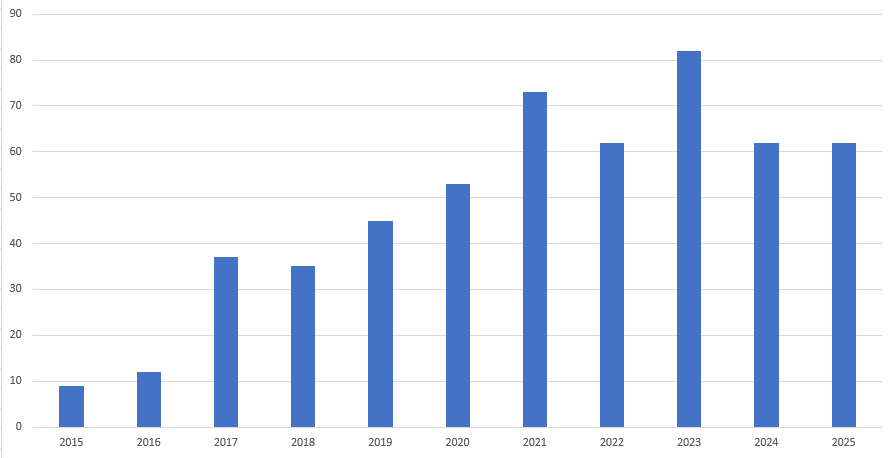
\includegraphics[width=\textwidth, height=6cm, keepaspectratio]{graficopublicacoes.png}
    \caption{Número de publicações ao longo dos anos durante o período pesquisado.}
    \label{fig:graficopublicacoes}
\end{figure}

\section{Características de processo}

% POLIDO%

O desempenho do processo de destilação por membranas é determinando pela interação entre as condições operacionais, as características da alimentação, as propriedades da membrana e a configuração do módulo~\cite{Gonzalez2017,Swaminathan2018}. Esses fatores influenciam diretamente os mecanismos de transferência de calor e massa e a estabilidade do processo~\cite{Eykens2016}. 

Além disso, fenômenors como polarização de temperatura e de concentração, incrustação e molhamento podem alterar progressivamente o desempenho da membrana durante a operação~\cite{Yao2020WettabilityMD, AbdelKarim2021, Hsieh2024ScalingWetting}.

Entre os fenômenos inerentes ao processo, a polarização de temperatura exerce influência direta sobre a força motriz para o transporte de vapor através da membrana. Observa-se que seus efeitos dependem tanto das caracteristicas hidrodinêmicas quanto das características do processo, onde membranas finas com maior permeabilidade e condutividade térmica mostraram-se mais suscetíveis à polarização de temperatura e aos efeitos decorrentes do aumento da salinidade~\cite{Eykens2016}.

Outro ponto focal é a interação entre a temperatura de operação em conjunto com elevanda salinidade, onde a polarização de temperatura pode promover uma pressão de vapor desfavorável ao transporte de vapor, em especial para módulos que operam com baixo número de reynolds no canal de alimentação. Em contrapartida, para membranas espessas as características morfológicas apresentam maior influência sobre o desempenho~\cite{Eykens2016}.

A configuração do módulo é outro fator determinante para o desempenho térmico e energético do processo, os quais variam em função da resistência a transferência de calor e massa inerente da configuração~\cite{Gonzalez2017,Swaminathan2018}. 

A comparação entre módulos de contato direto (DCMD) e módulos com espaçamento com permeado (PGMD) pode apresentar valores de gain output ratio (GOR) superiores aos obtidos em módulos com espaçamento de ar (AGMD) quando aplicados ao tratamento de soluções com baixa salinidade. Entretanto, essa diferença de desempenho decai consideravélmente com o aumento da salinidade, tornando o AGMD mais favorável para o tratamento de soluções com elevada salinidade~\cite{Swaminathan2018}.

O desempenho do módulo AGMD é dependente da espessura do espaçamento de ar e sua condutividade térmica, de modo que a redução da espessura e aumento da condutividade favorecem a produção de permeado. Entretanto o aumento da condutividade do espaçamento não deve estar atrelado ao aumento da condutividade da membrana, a qual intesifica as perdas de calor por condução. Outro ponto importante é o cuidado quanto a redução excessiva do espaçamento, o que pode transformar o módulo AGMD em PGMD, em função do possível acúmulo de permeado no espaçamento~\cite{Swaminathan2018}. 

Além das condições operacionais e da configuração do módulo, a hidrofobicidade da membrana é fundamental para a estabilidade do processo. Caso a membrana tenha uma redução de sua hidrofobicidade, ocorre o fenômeno de molhamento dos poros, podendo ocorrer de forma parcial ou completa, comprometendo a seletividade da membrana e reduzindo a qualidade do permeado~\cite{Yao2020WettabilityMD, AbdelKarim2021}.

A suscetibilidade ao molhamento depende da interação entre as propriedades superficiais da membrana, as condições hidrodinâmicas e a composição da água a ser tratada~\cite{Yao2020WettabilityMD}. Quanto a membrana, destacam-se rugosidade, molhabilidade, tensão superficial, tamanho dos poros, carga superficial, enquanto para o escoamento temos como principais fatores a velocidade, temperatura, direção do fluxo e gradiente de pressão como os principais fatores~\cite{Yao2020WettabilityMD}. Para a composição da água é possível destacar a concentração e natureza dos contaminantes, difusivade e pH~\cite{Yao2020WettabilityMD}.

Do ponto de vista do molhamento, o principal fator a ser observado é a pressão de entrada de líquido (Liquid Entry Pressure - LEP), a qual é calculada com base no maior diâmetro de poro presente na membrana, pelo ângulo de contato, tensão superficial do fluido e um fator de forma atribuido a geometria dos poros. A presença de surfactantes na água a ser tratada impacta diretamente o LEP, uma vez que reduz a tensão superficial da solução, facilitando a penetração nos poros~\cite{Yao2020WettabilityMD}. Desse modo, a avaliação da estabilidade do processo não deve considerar apenas as propriedades iniciais da membrana, mas também a interação entre a membrana e a solução ao longo do processo~\cite{Yao2020WettabilityMD}.

A molhabilidade da superfícia pode ser interpretada pelos modelos de Young, Wenzel e Cassie-Baxter, os quais dieferem quanto a interação líquido-superfície~\cite{Yao2020WettabilityMD}. Em particular o modelo de Cassie-Baxter associa o aprisionamento de ar entre o líquido e a superfície com a obtenção de superfícies super-hidrofóbicas e ominifóbicas. Para estas superfícies, a combinação entre elevada rugosidade e baixa tensão superficial propicia elevados ângulos de contato e baixos ângulos de inclinação~\cite{Yao2020WettabilityMD}.

Nesse sentido, membranas com ângulo de contato superior a 150° são classificadas como super-hidrofóbicas e podem ser obtidas por meio do aumento da rugosidade superficial, da criação de estruturas hierárquicas ou da redução da tensão superficial do material~\cite{Yao2020WettabilityMD}. 

Observou-se durante o processo de revisão bibliográfica o uso de diferentes estratégias para a obtenção de superfícies super-hidrofóbicas, como o uso de nanopartículas de sílica ou carbona, poduzindo superfícies com rugosidade multinível, apresentando propriedades hidrofóbicas e oleofóbicas~\cite{Laqbaqbi2017,Gong2019}. 

Em experimentos com módulo DCMD com soluções contendo diferentes salinidades e 1~$g/L$ de óleo mineral, observou-se fluxos de permeado entre 8 e 10~$L/m^2h$ durante 48 horas para salinidade próxima a água do mar. Entretanto para solução com salinidades maiores (98,5 e 167~$g/L$) o fluxo de permeado observado foi inferior a 1~$L/m^2h$, enquanto a rejeição a sal e óleo permaneceram elevadas, indicando que não houve a ocorrência de molhamento~\cite{Gong2019}.

Além do molhamento, a incrustação com matéria orgânica (fouling) e a com matéria inorgânica (scaling) prejudicam o processo, promovendo a redução gradual do fluxo de permeado através do aumento da resistência a transferência de massa e favorecendo a ocorrência de molhamento~\cite{AbdelKarim2021,Hsieh2024ScalingWetting,Du2023Antifouling}.

Para contaminantes orgânicos como o ácido húmico e polissacarídeos, pode ocorrer a formação de camadas na superfície da membrana, enquanto para os contaminantes inorgênicos há a dependência da ocorrência de supersaturação e polarização, exixtentes na superfície da membrana~\cite{Laqbaqbi2017,Du2023Antifouling}.

A interação entre diferentes contaminantes também intensifica a ocorrência de fouling, onde a presença de ácido húmico e Nacl propicia a formação de depósitos, facilitando a ocorrência de molhamento e do mecanismo de adsorção e dessorção, reduzindo a qualidade do permeado produzido~\cite{Laqbaqbi2017}. Quanto aos compostos inorgânicos, as características de processo podem promover a cristalização na superfície da membrana ou no escoamento~\cite{Laqbaqbi2017}, onde cristais em formato de agulha, geralmente formados ao longo do escoamento, podem promover scaling na superfície da membrana, propiciando o molhamento nos pontos de deposição~\cite{Hsieh2024ScalingWetting}.

A presença de compostos orgânicos voláteis (VOCs) na água a ser tratada reduz a qualidade do permeado produzido, uma vez que podem atravesar a membrana via adsorção-desorção ou como vapor, uma vez que apresentam temperaturas de ebulição inferiores a da água~\cite{Yao2018}.

A ocorrência de fenômenos como fouling e scaling exige o uso de estratégias de prevenção ou recuperação. Como prevenção, é possível citar técnicas como coagulação, flotação, micro e nanofiltração, osmose reversa e processos oxidativos avançados~\cite{Laqbaqbi2017,AbdelKarim2021}. 

Dentre estas técnicas, os processos oxidativos avançados destacam-se pela capacidade de remoção de surfactantes, reduzindo a propenção ao molhamento causada pela presença destes compostos~\cite{AbdelKarim2021}. O uso de pré-filtração favorece a remoção ou cristalização de contaminantes antes da chegada ao módulo, reduzindo a incidência de deposição de contaminantes na superfície da membrana~\cite{AbdelKarim2021}.

Quanto as técnicas de recuperação, procedimentos de limpeza podem recuperar de maneira parcial ou total o fluxo de permeado. Porém deve-se considerar o tipo de material depositado, uma vez que o uso de produtos químicos inadequados pode acarretar a degradação da membrana ou alteração de suas caracteristicas superfíciais~\cite{Laqbaqbi2017,AbdelKarim2021}. Outro ponto de atenção é a permanência de pontos de incrustação após o processo de limpeza, os quais prpiciam a ocorrência de novas deposições e podem atuar como pontes hidrofílicas, favorecendo a ocorrência de molhamento~\cite{AbdelKarim2021}.

O processo de caracterização da membrana, antes e após o uso, é uma etapa crucial para indentificar se a membrana escolhida possui as caracteristicas necessária para o processo e para compreender o impacto dos contaminantes presentes na água a ser tratada~\cite{Laqbaqbi2017}.

Entre as técnicas empregadas, a microscopia eletrônica de varredura (SEM), a microscopia de força atômica (AFM) e a porosimetria de fluxo capilar permitem avaliar a morfologia da superfície da membrana, analisando caracteristicas como rugosidade, porosidade, permeabilidade, formato e diâmetro de poro. Quanto a composição química dos contaminantes depositados na membrana, pode-se aplicar a espectroscopia ATR-FTIR ou espectroscopia por dispersão de energia (EDS)~\cite{Laqbaqbi2017}.


% BRUTO
%Os estudos sobre destilação por membranas indicam que o desempenho do processo é fortemente influenciado pelas condições operacionais e propriedades da membrana. Observa-se que membranas finas e com elevada permeabilidade são mais afetadas pela polarização de temperatura e aos efeitos da salinidade, enquanto a influência das características morfológicas é mais relevante em membranas espessas \cite{Eykens2016}.

%A literatura também destaca a importância da configuração do módulo no desempenho energético e operacional da destilação por membranas \cite{Gonzalez2017,Swaminathan2018}. Em geral, módulos DCMD (direct contact membrane distillation) e PGMD (permeate gap membrane distillation) apresentam maiores valores de gain output ratio (GOR) em baixas salinidades.

%Por outro lado, módulos AGMD demonstram melhor estabilidade para soluções mais concentradas. Entretanto, o uso de gaps reduzidos pode promover inundação por permeado condensado, comprometendo o desempenho do módulo em altas salinidades \cite{Swaminathan2018}.

%Diversos trabalhos abordam os mecanismos de molhamento e incrustação em membranas hidrofóbicas \cite{Yao2020WettabilityMD, AbdelKarim2021, Hsieh2024ScalingWetting}. O molhamento pode ocorrer de forma superficial, parcial ou completa, sendo favorecido pela presença de surfactantes e por incrustações na superficie da membrana \cite{Yao2020WettabilityMD, AbdelKarim2021}. Fatores como rugosidade, tamanho de poro, temperatura, velocidade de escoamento e composição do fluido exercem influência direta sobre estes fenômenos \cite{Yao2020WettabilityMD}.

%Os estudos também demonstram que membranas superhidrofóbicas, obtidas por modificações superficiais e aumento da rugosidade, apresentam maior resistência ao molhamento \cite{Yao2020WettabilityMD}. Em relação ao fouling (incrustações orgânicas) e scaling (incrustações inorgânicas), ambos reduzem progressivamente o fluxo de permeado e podem induzir o molhamento dos poros \cite{AbdelKarim2021, Hsieh2024ScalingWetting}.

%A literatura também aponta que procedimentos de limpeza química podem recuperar parcialmente o fluxo de permeado, embora possam causar degradação estrutural da membrana e favorecer novos pontos de nucleação para incrustações \cite{AbdelKarim2021}. 

%Estratégias de fabricação também vêm sendo estudadas para aumentar a estabilidade térmica e reduzir o inchamento das membranas. O uso de álcool isoamílico como banho de coagulação em membranas de PVDF resultou em membranas mais resistentes ao molhamento e com fluxos estáveis durante ensaios de dez dias \cite{Nguyen2025MDStability}.

%O estudo \cite{Eykens2016} (2016) trata da influencia das características do escoamento e da membrana no fluxo de permeado. Indica que a polarização de temperatura é mais forte em membranas finas, com alta permeabilidade e alta condutividade térmica. Além disso, verificou-se que o aumento da salinidade afeta de modo mais significativo membranas mais finas. 

%Dependendo das temperaturas de operação empregadas, o efeito combinado da polarização de temperatura e da elevada salinidade pode levar à formação de diferença de pressão negativa, especialmente com baixos números de Reynolds. Além disso, observa-se que as membranas mais finas são mais influenciadas pelas características do processo enquanto as membranas mais grossas são mais influenciadas pelas características morfológicas.

%O artigo \cite{Gonzalez2017} (2017) apresenta uma revisão ampla sobre os métodos de destilação por membrana, abordando o equacionamento da transferência de calor e massa para as principais configurações. É apresentado uma tabela com os principais agentes de incrustração em MD (Alcalinos, não alcalinos, particulados, orgânicos e biológicos).

%Os autores \cite{Swaminathan2018} (2018) citam o uso do próprio fluido de alimentação como corrente fria do módulo, permitindo seu pré-aquecimento durante a passagem pelo sistema. Os autores apresentam o equacionamento para a quantificação do custo de produção de água em MD, indicando que, na maioria dos estudos, o custo com aquecimento não é considerado devido ao reaproveitamento de calor.

%O estudo indica que o gain output ratio (GOR) para módulos DCMD e PGMD é superior ao de módulos AGMD para baixas salinidades, porém apresenta rápida redução com o aumento da salinidade. O artigo esclarece que aumentar a condutividade do gap aumenta na produtividade, e que o mesmo não deve ser entendido com aumentar a condutividade da membrana, a qual aumenta a perda de calor, e ambos não estão diretamente correlacionados. 

%Os autores apontam limitação na aplicação em larga scala de módulos CGMD, uma vez que estes módulos utilizam um gap muito pequeno (proximo de zero) ou espumas metálicas como espaçadores, o que provoca uma grande perda de carga, dificultando a saída do permeado. O airgap é tratado como uma membrana mais espessa, de modo a apresentar baixa condutividade térmica e alta permeabilidade, características que facilitam a obter um maior GOR para altas salinidades. 

%O desempenho do módulo CGMD se aproxima do AGMD para baixos fluxos e alto GOR quando se utiliza uma membrana mais espessa. O artigo expõe que AGMD é o módulo promissor para tratamento de altas salinidades, mas ressalta que um gap pequeno (aprox 1mm) pode ser inundado pelo permeado gerado, alterando o módulo para PGMD, o qual não performa bem em altas salinidades.

%Os autores de \cite{Yao2020WettabilityMD} (2020) descrevem as diferentes condições de molhamento de membranas.  Destaca que componentes não voláteis podem passar através da membrana através de "adsorção-desorção-adsorção". 

%O estudo aponta que a presença de surfactantes facilita o molhamento uma vez que eles reduzem localmente a tensão superficial do fluido, facilitando a penetração no poro (redução da pressão de entrada de líquido (LEP)). Os principais fatores que influenciam o molhamento e o fouling são: as características superficiais da membrana (rugosidade, molhabilidade, tensão superficial, tamanho de poro, carga da superficie e grupo funcional), as características hidrodinâmicas do processo(velocidade, temperatura, direção, gradiente de pressão) e as características do fluido(fração molar, difusividade, carga, ph e natureza dos contaminantes). 

%O ângulo de contato é descrito através de três modelos, Young, Wenzel e Cassie-Bexter, que diferem quanto ao grau de penetração do líquido na superfície. O artigo também apresenta o ângulo de inclinação (tilt angle) como uma forma para avaliar a molhabilidade do material. Ressalta-se que o regime de Casie-Bexter é essencial para membranas superhidrofóbicas e ominifobicas, permitindo alto ângulo de contato e baixo tilt angle, associados à combinação de baixa tensão superficial do material e do fluido e alta rugosidade. 

%Para membranas com topologia hierárquica, o aumento do ar aprisionado reduz significativamente a dependência das propriedades intrínsecas do material para a repelência de líquidos. 

%O artigo classifica como membranas superhidrofóbicas aquelas que possuem ângulo de contato superior a 150°, podendo ser obtidas através do aumento da rugosidade superficial com estrutura hierarquica ou diminuindo a tensão superficial do material da membrana.

%O artigo \cite{AbdelKarim2021} (2021) descreve o fenomeno de molhamento em três estágios: superficial, parcial e completo. O trabalho aborda principalmente os aspectos sobre incrustação de matéria orgânica (fouling), aos pré tratamentos aplicáveis e às técnicas para recuperação de membranas. 

%O estudo compara a redução no fluxo de permeado em função de diferentes tipos de contaminantes e exibe imagens sobre diferentes tipos de deposições sobre a superfície da membrana. 

%Os autores destacam o uso de processos oxidativos avançados (AOPs) para controlar a presença de surfactantes, reduzindo o potencial de molhamento. Também é indicado o uso de pré filtros para atuarem como cristalizadores antes da entrada do módulo. O trabalho aponta que o uso de anti incrustantes é economicamente mais vantajoso do que o uso de ácidos, mas que em certos casos pode intensificar incrustações orgânicas. 

%O artigo ressalta que o processo de limpeza química é capaz de recuperar o fluxo de permeado mas pode deteriorar a membrana, seja pela ação quimica ou pelas características dos depósitos formados. Além disso, depósitos residuais podem agir como "pontes hidrofílicas" ou servir de ponto de nucleação para novos depósitos.  

%O estudo \cite{Hsieh2024ScalingWetting} (2024) aborda a análise do mecanismo de incrustação de matéria inorgânica (scaling) em membranas. %Utilizou-se um módulo VMD, com microscópios monitorando ambos os lados da membrana e sensores em linha para acompanhar a condutividade e turbidez
%Relizou-se experimentos com carbonato de calcio, silica e gipsita (gesso), utilizando uma membrana de PTFE. 

%A alimentação foi mantida a 50~$^\circ$C e utilizou-se vácuo de 15,6~KPa. O estudo conclui que o fenômeno de molhamento está associado a incrustação cristalina, podendo ser intensificado mediante a deposição de cristais com formato de agulha, os quais em geral se formam no escoamento. %Observa-se também que o fenômeno de incrustação está fortememnte relacionado ao tipo de espaçador utilizado no canal do módulo, uma vez que este influencia diretamente as características hidrodinâmicas do escoamento, favorecendo ou dificultando a deposição de sais.

%Os autores de \cite{Nguyen2025MDStability} (2025) abordam o uso de álcool isoamílico como banho de coagulação para a produção de membranas de PVDF, com o objetivo de gerar membranas mais resistentes a altas temperaturas. Para os experimentos utilizou-se um módulo DCMD, operando com temperaturas de 65~$^\circ$C e 20~$^\circ$C no lado quente e frio, respectivament, utilizando água deionizada no lado frio e água do mar com e sem pré tratamento no lado quente. Utilizou-se uma membrana de PVDF, apresentando espessura de 268~$\mu m$, diâmetro médio de poro de 0,31~$\mu m$, ângulo de contato de 152° e porosidade de 84~\%. 

%Os experimentos com duração de 10 dias demonstraram que a membrana produzida com álcool isoamílico apresentou fluxo de permeado de aproximadamente 19~$Lm^{-2}h^{-1}$. Entretanto, observou-se redução decorrente de incrustação no experimento que utilizou água do mar não filtrada, reduzindo para 14,4~$Lm^{-2}h^{-1}$. Observou-se também um aumento na concentração de sólidos totais dissolvidos de 37 para 45~$mgL^{-1}$ ao longo do experimento.  

%O artigo conclui que o uso de álcool isoamílico reduz a ocorrência de inchamento da membrana, provocado pela evaporação de resíduos do solvente utilizados no processo de fabricação e aprisionados no interior da estrutura da membrana. %Além disso, as membranas produzidas com álcool isoamílico apresentaram maior fluxo de permeado quando comparadas às produzidas utilizando água ou etanol como banho de coagulação.

%Resumo

%O artigo \cite{Laqbaqbi2017} (2017) inicia comentando sobre as principais caracteristicas necessárias para as membranas para o processo MD, como alto LEP e porosidade, baixa condutividade térmica e espessura. O artigo indica o uso de uma fina camada de polimero hidrofílico, de modo a previnir o molhamento e incrstação provocados pela presença de óleo na alimentação. O artigo também comenta sobre testes realizados em membranas hidrofóbicas e óleofóbicas, as quais são fabricadas a partir de nanofibras de PVDF-HFP enxertadas com nanopartículas de sílica carregadas negativamente, apresentando resistência ao molhamento para soluções com baixa tensão superficial como óleo mineral, decano e etanol. 

%O artigo destaca que a incrustação na superfície da membrana atua tanto pelo bloqueio dos poros como também pelo aumento da resistência a transferência de massa. É destacado que o ácido húmico interage através do mecanismo de adsorção-desorção, adentrando os poros e promovendo o fenômeno de molhamento. Também é comentado que a interação entre o ácido húmico e NaCl favorece a ocorência de incrustações. 

%O artigo comenta sobre as formas de deposição de compostos inorgânicos, os quais são mais influenciados pela polarização de temperatura e concentração, onde sais que perdem solubilidade com o aumento da temperatura tem tendência a cristalizarem na região central do escoamento e não na superfície da membrana. Já os saia que tem aumento da solubilidade com a temperatura tendem a cristalizar na superfície da membrana, como o NaCl.

%O artigo indica que SEM é uma das principais técnicas utilizadas para caracterização de membranas por microscopia, atuando tanto na superfície como na seção transversal. Entretanto o preparo para SEM afeta a camada de incrustante, limitando a caracterização dos contaminantes. Também é comentado o uso de AFM (microscopia de força atômica) para avaliar rugosidade, diâmetro de poro médio e distribuição, porosidade.

%Outra técnica comentada é a ATR-FTIR, a qual permite obter informações sobre a composição química dos incrustantes sem a necessitade de uma preparação da amostra.

%O artigo indica o uso de diferentes técnicas de pré tratamento como coagulação, flotação, MF/NF/RO e antiencrustantes como formas de evitar encrustações. Também é comentado o uso de HCl em concentrações entre 2-5 wt\% para a limpeza da superfície das membranas, recuperando completa ou parcialmente o fluxo de permeado inicial. Também é comentado que o químico utilizado para o processo de limpeza deve ser escolhido de acordo com o tipo de encrustante presente na água (orgânico, inorgânico ou biológico).

%O artigo \cite{Yao2018} (2018) aborda o impacto da presença de compostos orgânicos voláteis na água de produção proveniente da exploração de reservatórios de gás natural, com enfoque para o acido acético (de ocorrência natural), alcool isopropilico, 2-Butoxietanol, etilenoglicol (compostos adicionados à água de fraturamento). O artigo utilizou membranas de PVDF de fibra oca em um módulo VMD, as quais possuem diâmetro médio de 0,1 $\mu$m, 63\% de porosidade e LEP de 2,3 bar. A solução foi bombeada a 400 ml/min a uma temperatura de 70~$^\circ$C e uma pressão de vácuo de 850 mbar.

%O artigo observa a cocorrência do mecanismo de adsorção-desorção para os compostos 2-Butoxietanol e ácido acético, explicando a passagem destes compostos sem que ocorra o molhamento da membrana, principalmente no caso do 2-Butoxietanol, o qual apresentou uma mobilidade muito superior a da água, mesmo possuindo uma temperatura de ebulição maior e uma pressão de vapor menor. As concentrações de surfactantes empregadas no estudo não foram significantes para reduzir a tensão superficial da solução, de modo que também não afetou o LEP, não afetando a resistência ao molhamento da membrana. o autor indica que a queda no fluxo de permeado nos experimentos de 72 horas foi decorrente do molhamento parcial dos poros. O artigo conclui que o transporte de VOCs pela membrana se dá tanto pela evaporação, da memsa forma que o vapor d'água, quanto pelo mecanismo de sorção-desorção, onde a ligação entre as moléculas do VOC e do vapor d'água promovem o carreamento do VOC pelo poro da membrana, promovendo o molhamento dos poros em processos de longo prazo.


%O artigo \cite{Gong2019} (2019) O artigo utiliza uma membrana plana de PVDF como base para produzir uma membrana monificada com nano partículas de carbono, resultando uma rugosidade multinível, oleofóbica e hidrofóbica. Os experimentos foram conduzidos considerando uma vazão de 3 mL/min na alimentação e 6 mL/min no permeado, operando como DCMD. Considerou-se na alimentação diferentes salinidades de 3,25, 9,85 e 16,7 wt\% e com 1~g/L de óleo mineral. Como o aquecimento foi realizado utilizando a luz solar, a temperatura da alimentação este em 40~$^\circ$C e 50~$^\circ$C para o caso com alta incidência solar. Para água do mar, a membrana apresentou bom fluxo (entre 8 e 10 L/m2h) durante 48 horas, entretanto para contaminação de óleo e nas salinidades maiores, apresentou fluxo muito baixo, inferior a 1L/m2h. Apesar disso manteve alta rejeição de sal e óleo, sem indicativos de molhamento nas 48 horas.

%O artigo \cite{Du2023Antifouling} (2023) explora os tipos de encrustantes que atuam sobre membranas em diferentes industrias. Para MD, resaltasse na na industria de óleo e gás a presença de oléo diesel, NaCl, magnésio, silica, silicato e fosfatos. O artigo indica que a ocorrência de encrustação por matéria inorgênica na superfície da membrana é maior por conta do efeito de polarização de temperatura. Os encrustantes orgânicos, principalmente ácido húmico e polissacarídios, geralmente formam uma primeira camada com aspecto de gel, em função da elevada hidrofobicidade das membranas empregadas em MD. O artigo cita a ocorrência de sorção-desorção do ácido húmico, promovendo redução do fluxo sem a ocorrência de molhamento. O artigo cita o uso de materiais hidrofóbicos, com elevada rugosidade superficial(estrutura com reentranças) ou modificados com materiais com baixa energia superficial como maneiras de reduzir a ocorrência de incrustações. Indica o uso de membranas Janus, as quais possuem superfície com molhabilidade asimétrica. O artigo também cita o uso de técnicas para evitar encrustações, como borbulhamento e ultrasom.


\section{Tratamento de água}

% POLIDO

A aplicação da destilação por membranas ao tratamento de diferentes matrizes aquosas tem sido avaliada através de estudos envolvendo diversos efluentes industriais, os quais avaliam a influência da composição da água a ser tratada na performance do processo~\cite{Gueccia2021HClReco
very,Su2017,RuizAguirre2019PermeateQuality,Woo2021ElectrospunMD,Su
ga2021VMD,Kujawa_PVDF_SWCNH,Abdelrazeq2022DCMD,Adham2023}. 

O uso de um módulo AGMD para a concentração de ácido clorídrico oriundo do processo de decapagem associado à galvanização a quente ilustra a capacidade do processo de lidar com efluentes industriais complexos~\cite{Gueccia2021HClRecovery}. Utilizou-se no estudo uma unidade piloto associada a etapas de pré-tratamento, operando durante oito horas, com temperaturas de 60~$^\circ$C~e 25~$^\circ$C nos lados quente e frio, respectivamente. Através do processo obteve-se a recuperação de 15 a 26\% da água presente na solução de ácido clorídrico tratada.

A avaliação da influência de caracteristicas da membrana empregada na qualidade/estabilidade do processo pode ser realizada mediante a comparação entre membranas virgens e modificadas. Para o tratamento de uma solução com 35~$gL^{-1}$ em um módulo DCMD, empregou-se membranas de PVDF com e sem nanopartículas de sílica, onde as membranas com 

--------Parei aqui-----------

% BRUTO

\cite{Gueccia2021HClRecovery} - 2021 - O autor aborda o uso de um módulo AGMD para concertação de ácido clorídrico, o qual é o oriundo do proceso de decapagem do processo de galvanização a quente. Apesar de não tratar diretamente sobre água de produção, expõe a capacidade do processo de operar com fluidos complexos. Para o estudo utilizou-se uma unidade piloto, a qual operou com pré tratamentos como filtragem, separador de óleo, filtragem com carvão ativado e diálise por difusão. O estudo teve duração de 8 horas, operando com temperaturas de 60~°C e 25~°C no lado quente e no lado frio, respectivamente.

O artigo \cite{Su2017} (2017) avaliou o desempenho de uma membrana de PVDF em um módulo DCMD com duração de 100 horas, utilizando salmoura com concentração de 35~$gL^{-1}$ a 50~$^\circ$C na alimentação e água deionizada a 10~$^\circ$C no lado frio. A membrana de PVDF original apresentou fluxo inicial de 17~$Lm^{-2}h^{-1}$, apresentando redução após a oitava hora de experimento enquanto a membrana de PVDF modificada com nanopartículas de sílica com concentração de 7,47~\% apresentou fluxo praticamente constante de 25~$Lm^{-2}h^{-1}$ ao longo de todo o experimento.

A condutividade do permeado da membrana de PVDF origial apresentou aumento após a vigésima hora de experimento, finalizando com valor próximo de 35~$\mu Scm^{-1}$. A condutividade da membrana de PVDF modificada apresentou um aumento da condutividade do permeado muito inferior, finalizando o experimento com 5~$\mu Scm^{-1}$. 

O experimento com apenas a superfície da membrana modificada com nanopartículas de sílica apresentou fluxo de permeado semelhante ao da membrana com nanopartículas de sílica em toda composição, entretanto apresentou um pico de condutividade após 95 horas de experimento, indicando a ocorrência de molhamento parcial da membrana.

O estudo \cite{RuizAguirre2019PermeateQuality} (2019)  realiza experimentos com três módulos comerciais, avaliando o tratamento de salmouras de 35 a 140~g/L. Os módulos utilizados eram PGMD e V-AGMD, operando com temperaturas de entrada do lado quente entre 60 e 80~$^\circ$C, e no lado frio de 20 a 30~$^\circ$C. Foram realizados experimentos de curto prazo (75 minutos, após um período transiente de 25 minutos), nos quais se observou que, após as interrupções, ocorre um pico de salinidade, a qual o autor atribui a um possível molhamento. Observou-se que não ocorre o pico de condutividade no retorno a operação caso o módulo seja mantido com água deionizada durante o período de intervalo.

Os autores de \cite{Woo2021ElectrospunMD} (2021) avaliam o uso de membranas planas produzidas através do processo de eletrofiação feitas de PVDF-co-HFP e aerogel de sílica, aplicadas em um sistema AGMD. As membranas apresentaram espessura de 140$\mu m$, diâmetro médio de poro de 0,39 $\mu m$, porosidade de 90~\%, LEP de 1,91~Bar, ângulo de contato de 166° e ângulo de escorregamento de 3,5°. Os experimentos foram realizados utilizando uma solução com 35~g/L de NaCl, com uma temperatura do lado quente de 60°C e 20°C no permeado. 

O experimento teve duração de 31 dias, mantendo fluxo estável de aproximadamente 10~$Lm^{-2}h^{-1}$ e indíce de rejeição de sal de 99,99~\%. Análise de SEM não observou a ocorrência de incrustação, sendo a estabilidade do processo atribuída ao baixo ângulo de escorregamento apresentado pela membrana. 

O artigo \cite{Suga2021VMD} (2021) avalia a aplicação de um módulo VMD utilizando membranas de fibra oca de PVDF, com espessura de 280~$\mu m$, diâmetro de poro médio de 0,10~$\mu m$, porosidade de 72~\%, ângulo de contato de 132° e LEP de 0,37~bar. Nos experimentos, utilizou-se uma salmoura com 35~g/L, operando com temperatura de 65~$^\circ$C para o lado quente e 20~$^\circ$C para o lado frio,  e utilizando vazões de 7~$Lmin^{-1}$ e 10~$Lmin^{-1}$ no lado quente e no lado frio, respectivamente. 

O experimento de longo prazo durou 330 horas, iniciando com fluxo de permeado de 19,3~$Lm^{-2}h^{-1}$ e mantendo 87~\% do fluxo de permado inicial, além de condutividade inferior a 8 $\mu S/cm$. Os autores enfatizam que o LEP está diretamente relacionadol a capacidade de rejeição de sal e estabilidade do fluxo de permeado ao longo da operação. 

O artigo \cite{Kujawa_PVDF_SWCNH} (2021) investiga o uso de nanocornes de carbono (estruturas de carbono com formato cônico) para melhorar a superfície de membranas de PVDF aplicadas ao processo AGMD. A aplicação gerou superfícies super-hidrofóbicas, com ângulo de contato de até 165°, proporcionando uma melhora de 27~\% no fluxo de permeado quando em comparação com PVDF original. Os experimentos foram realizados utilizando uma salmoura com concetração de aproximadamente 29~g/L, com duração de 60 horas, utilizando temperatura do lado quente de 54~$^\circ$C e do lado frio de 9~$^\circ$C.

Os autores de \cite{Abdelrazeq2022DCMD} (2022) avaliam o uso de um membrana de PE em um módulo DCMD para o tratamento de água mimetizada com as características do rejeito de uma planta de dessalinização térmica localizada no Qatar. A membrana utilizada possui distribuição de poros entre 0,3 e 0,7~$\mu m$ e espessura de 15,5~$\mu m$.

Os experimentos consideraram duas concentrações diferentes, uma com 25,2 e outra com 75,5~$gL^{-1}$, composta por sódio, magnésio, cálcio, potássio, estrôncio, boro, cloreto, sulfato, bicarbonato e brometo. Também utilizou-se ácido húmico com concetrações de 15, 25, 35 e 45~$mgL^{-1}$ para avaliar a ocorrência de incrustações na superfície da membrana. 

Os experimentos tiveram duração de 100 horas, com temperatura do lado quente foi de 70~$^\circ$C e do lado frio de 20~$^\circ$C, realizando interrupções a cada 20 horas para avaliar o estado da membrana. 

A rugosidade superficial da membrana no início do experimento era de 81,39~nm, alcançando 357,1~nm após 100 horas de experimento, decorrente da incrustação. Observou-se uma redução de 94~\% do ângulo de contato após o experimento, o que provocou uma queda considerável no indíce de rejeição de sal após 60 horas de experimento, indicando a ocorrência de molhamento.

O fluxo de permeado apresentado inicialmente foi de aproximadamente 120 e 135~$Lm^{-2}h{-1}$ para a salmoura mais concentrada e menos concentrada, respectivamente, reduzindo-se a 16 e 28~$Lm^{-2}h{-1}$ ao final do experimento. 

Nos experimentos com ácido húmico apresentaram taxa de rejeição superior a 98,5~\%, embora com queda no fluxo de 51~\%. A incrustação provocada pôde ser facilmente contornada mediante lavagem com água, recuperando o fluxo de permeado em 95~\%.

O artigo \cite{Adham2023} (2023) aborda inicialmente a comparação entre dois módulos comerciais de destilação por membranas, um VMD e outro AGMD, para o tratamento de água residual do processo de dessalinização térmica de uma planta no Qtar. A água residual apresentou TDS de 71~$mgL^{-1}$, a qual foi pré tratada com um sistema de filtração composto de um filtro de 1~$\mu m$ e um filtro de carvão ativado. O módulo AGMD apresentou redução do fluxo de permeado de aproximadamente 37~\% nos primeiros dias do experimento, o que levou a interrupção. O módulo VMD apresentou fluxo de permeado de aproximadamente 4,5~$Lm^{-2}h^{-1}$, com condutividade próxima a 1~$\mu Scm^{-1}$ nos primeiros dois dias, e próxima a 10~$\mu Scm^{-1}$ nos oito dias restantes de experimento. Utilizou-se temperatura da alimentação em 32~$^\circ$C, com vazão de 1,4~$Lmin^{-1}$ e vácuo de 70 $mbar$. 

Posteriormente, realizou-se o experimento sem considerar o pré tratamento da água, o que resultou em redução do fluxo de permeado de 5 para aproximadamente 3,8~$Lm^{-2}h^{-1}$ ao longo de seis dias de experimento, indicando a ocorrência de incrustação. A condutividade apresentou aumento abrupto a partir do quarto dia de experimento, indicando a occorencia de molhamento de poros. Observou-se que o molhamento ocorreu devido a presença de um agente antiespumante presente na água, o qual havia sido removido durante a etapa de pré tratamento.

A segunda etapa do artigo utilizou o módulo VMD acoplado com um sistema de umidificação-desumidificação para compor um sistema de descarga líquida zero. A tratada possuia TDS de 63~$mgL^{-1}$, a qual foi direcionada para uso em um sistema de fraturação hidráulica. O sistema apresentou fluxo de permeado contante de aproximadamente 5~$Lm^{-2}h^{-1}$, com condutividade próxima de 10~$\mu Scm^{-1}$ durante as 30 horas de experimento. Os autores relatam que em função dos aditivos químicos terem passado a tolerar niveis de salinidade maiores, a aplicação do processo para dessalinização de água para o processo de fraturamento hidráulico se tornou dispensável.

\section{Tratamento de água de produção}

%\textcolor{red}{FALAR SOBRE OS ARTIGOS QUE ABORDAM O USO DE MD  PARA O TRATAMENTO DE ÁGUA DE PRODUÇÃO}

Os estudos relacionados ao tratamento de água salina e rejeitos de dessalinização demonstram que a composição da alimentação exerce forte influência sobre o desempenho do processo \cite{Abdelrazeq2022DCMD} . Ensaios utilizando rejeitos de dessalinização térmica mostraram que elevadas concentrações salinas favorecem a formação de incrustações e reduzem o ângulo de contato da membrana, promovendo molhamento parcial dos poros \cite{Abdelrazeq2022DCMD} . 

A aplicação da destilação por membranas no tratamento de água de produção tem demonstrado potencial para remoção de contaminantes orgânicos e sais presentes em água residual da indústria do petróleo \cite{Singh2011DCMD, Nawaz2021FO_MD, Pawar2022AGMD}. Os estudos relatam elevada rejeição de compostos orgânicos e baixa condutividade do permeado, mesmo em soluções contendo fenóis, cresóis, ácidos orgânicos e sais dissolvidos \cite{Singh2011DCMD}.

Sistemas híbridos integrando osmose direta e destilação por membrana também vêm sendo investigados para recuperação de água e regeneração da solução osmótica \cite{Nawaz2021FO_MD}. Nesses sistemas, observou-se que elevadas concentrações de óleo e graxa favorecem a formação de incrustações e o bloqueio de poros, especialmente por silicatos de cálcio, a qual pode ser evitada com a utilização de EDTA(ácido etilenodiamino tetra-acético) \cite{Nawaz2021FO_MD}.

Estudos em escala laboratorial e piloto indicam que o pré-tratamento da água de produção exerce papel fundamental na estabilidade operacional do processo \cite{Pawar2022AGMD}. Estratégias envolvendo filtração, ajuste de pH e oxidação química reduziram significativamente a ocorrência de incrustações e permitiram operação estável mesmo em elevadas salinidades por até 120 horas \cite{Pawar2022AGMD}. 

Em condições sem pré-tratamento adequado, observou-se redução gradual do fluxo de permeado, aumento da queda de pressão e aumento abrupto da condutividade do permeado, indicando molhamento da membrana e incrustação \cite{Pawar2022AGMD}. Os trabalhos também demonstram que o tratamento de água com elevada salinidade (255~$gL^{-1}$) favorece a precipitação de sais, principalmente cloreto de sódio, com menor contribuição de sulfato de estrôncio e hidróxido de ferro \cite{Pawar2022AGMD}. 

O artigo \cite{Hsieh2021Pretreatments} (2021) os autores realizaram experimentos para entender encrustações orgânicas e inorgânicas(fouling e scaling) em MD tratando água de produção real. Utilizou-se um módulo VMD e testaram-se 4 pré tratamentos: filtração, coagulação, flotação(induzida e com ar dissolvido) e oxidação. Utilizou-se membranas planas de PTFE com 0,2~$\mu m$ de espessura. A água de produção foi coletada de um poço de fraturamento hidráulico no Texas. O teste com água de produção retirada da cabeça do poço mostrou que a membrana apresentou molhamento instantaneamente, provocando entrada de PW na linha de permeado. Esse efeito foi atribuido a presença de alta concentração de hidrocarbonetos. O experimento com água de produção tratada na plataforma apresentou forte declinio nas primeiras 3 horas de experimento (vazão de alimentação de 1,2 L/min e pressão de 26 inHg) obtendo vazões iniciais de 60,40 e 28 L/m2h para temperaturas de 60, 50 e 40~$^\circ$C, respectivamente. Os autores atribuem a queda rápida no fluxo de permeado a adsorção de compostos orgânicos na superfície da membrana. Foram realizados testes de cinco dias com as duas amostras de água de produção tratadas na plataforma, com temperatura de alimentação de 50~$^\circ$C, vazão de 1,2L/min e pressão de 26 inHg. Para a PW com menor salinidade (T1), o teste apresentou fluxo com baixa redução, inferior a 12\%, e boa condutividade do permeado, menor que 500~$\mu S/cm$. Os teste com a PW de maior salinidade(T2) apresentaram um declinio rápido do fluxo de permeado nas primeiras 24 horas, finalizando o experimento no segundo dia em função da ocorrência de molhamento. Os autores indicam que a concentração maior de calcio e magnésio da PW T2 levou a acereleração de encrustação de inorgânicos, auxiliando na ocorrência de molhamento. Dentre os pré tratamentos que foram testados, a ultra filtração foi a que apresentou melhor desempenho, reduzindo a turbidez, os sólidos suspensos totais e o ferro.

Os autores de \cite{Singh2011DCMD} (2011) analisaram o uso de um módulo de pervaporação adaptado para operar como DCMD para o tratamento de água mimetizada com componentes semelhantes a água de produção oriunda do processo de Steam Assisted Gravity Drainage (SAGD), utilizado para recuperação de poços de petróleo para extração de óleo pesado e betume. 

O módulo emprega uma membrana de PTFE com diâmetro de poro nominal de 0,03~$\mu m$, espessura de 24~$\mu m$ e porosidade de 65~\%. Em fução da temperatura de trabalho escolhida, entre 100~$^\circ$C e 128~$^\circ$C para o lado quente e 20~$^\circ$C para o lado frio, utilizou-se um suporte de aço inoxidável poroso, com 6~mm de espessura. Os experimentos tiveram duração de 3 horas. %A figura \ref{fig:moduloSingh2011DCMD} apresenta o módulo utilizado no artigo.

\begin{figure}[H]
    \centering
    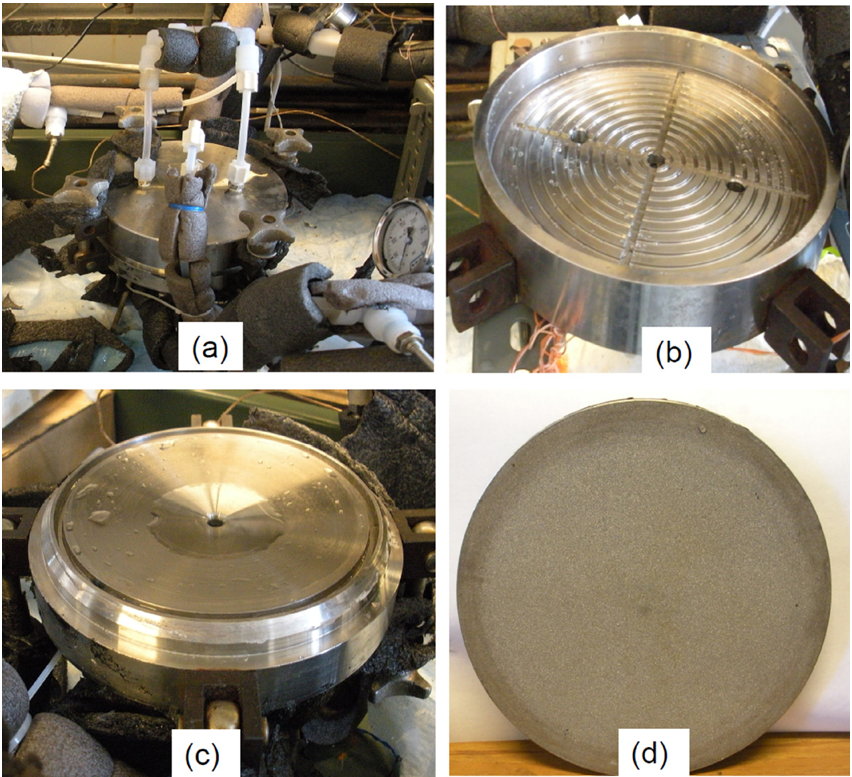
\includegraphics[width=\textwidth, height=11cm, keepaspectratio]{moduloSingh2011DCMD.png}
    \caption{Módulo DCMD utilizado no artigo \cite{Singh2011DCMD}: a) Módulo montado, b) Parte superior do módulo, c) Parte inferior do módulo e d) Suporte da membrana.}
    \label{fig:moduloSingh2011DCMD}
\end{figure}



A água de produção mimetizada continha 0,045~$gL^{-1}$ de fenol,  0,045~$gL^{-1}$ de cresol, 0,01~$gL^{-1}$ de ácido naftênico e 3~$gL^{-1}$ de cloreto de sódio. Para temperatura do lado quente de 128~$^\circ$C, observou-se um fluxo de permeado de 195~$Lm^{-2}h^{-1}$, sem aumento na condutividade do lado frio.

O estudo \cite{Macedonio2014_MD_ProducedWater} (2014) investiga a aplicação de módulos DCMD com membranas de fibra oca no tratamento de água de produção, empregando tanto membranas comerciais de polipropileno (PP) quanto membranas de PP e PVDF preparadas em laboratório. 

O trabalho não especifica a origem da água de produção, limitando a caracterização do efluente a parâmetros como sólidos dissolvidos totais (TDS), carbono total (TC), sólidos suspensos totais (TSS), condutividade, pH e 1,2-diethoxy ethane. Como etapa de pré-tratamento, foram utilizadas microfiltração e adsorção em carvão ativado. 

Os resultados indicaram rejeição superior a 99\% ao longo de um período experimental de sete horas. Além disso, foram observados comportamentos típicos do processo de DCMD, como a variação do fluxo de permeado em função de parâmetros operacionais, especialmente temperatura, concentração e vazão.

O artigo \cite{Nawaz2021FO_MD} (2021) aborda o uso de um sistema acoplado de osmose direta e DCMD para o tratamento de água de produção oriunda de diferentes estágios, incluindo água do processo de dessalinização do petróleo, água tratada para reinjeção, água do separador trifásico e rejeito de osmose reversa. 

Para o estudo, foram utilizadas águas mimetizadas com características semelhantes a amostras recolhidas de um campo de petróleo não identificado, considerando sais, metais, óleo e graxa, mas não foi mencionada a presença de orgânicos voláteis como os BTEX. 

Utilizou-se a água tratada para reinjeção como a solução extratora do processo de osmose direta, enquanto as demais fontes foram utilizadas como solução de alimentação. O módulo DCMD foi utilizado para regenerar a solução extratora, removendo permeado e elevando novamente sua pressão osmótica. Utilizou-se uma membrana hidrofílica de poliamida para o processo de osmose direta e PTFE com suporte em PP para o processo de destilação por membrana. 

Após os experimentos, as membranas utilizadas no processo DCMD foram caracterizadas através de microscopia eletrônica de varredura e espectrocopia de raios-x por dispersão de energia. Para isso foram armazenadas duas amostras, uma seca com ar seco e outra seca com ar seco e posteriormente mergulhada em água deionizada por dois minutos. O sistema integrado FO-DCMD operou com temperatura do lado quente de 60~°C e 20~°C do lado frio, ambos com vazão de 315~mL/min. 

Observou-se uma correlação entre o fluxo de permeado no módulo DCMD e o fluido utilizado como alimentação da osmose direta. A água do separador trifásico apresentou um menor fluxo, decorrente da maior concentração de óleo e graxa (entre 4 e 6 vezes mais que os outros fluidos). 

Também foi observado que a principal causa de incrustação no módulo DCMD foi o bloqueio de poros por silicato de calcio, o qual foi combatido através da adição de EDTA (ácido etilenodiamino tetra-acético), o que possibilitou a recuperação do fluxo inicial. 

Os experimentos foram encerrados ao apresentar fluxo de permeado inferior a 2~$Lm^{-2}h^{-1}$, apresentando duração entre 15 e 30 horas, para rejeito de osmose reversa e água do processo de dessalinização do petróleo, respectivamente. Para a água oriunda do separador terciário, observou-se um aumento da condutividade do permeado a partir de 13 horas, indicando molhamento parcial da membrana.

O artigo \cite{Pawar2022AGMD} (2022) estuda o tratamento de água de produção de um poço localizado no Texas (Estados Unidos), por meio de ensaios em escala de bancada, com um módulo DCMD, e em escala piloto com AGMD. Em ambos os casos utilizou-se membranas de PTFE com suporte em PP. Adotaram-se as condições operacionais de 60~$^\circ$C no lado quente e 20~$^\circ$C no lado frio para o módulo DCMD e 70~$^\circ$C no lado quente e 23~$^\circ$C no lado frio para o módulo AGMD. As vazões foram de 0,04554~$m^3/h^{-1}$ na escala de bancada e de 1,4~$m^3/h^{-1}$ na escala piloto. 

Nos ensaios laboratoriais, a água de produção foi filtrada com um filtro de 0,22~$\mu m$ para remoção de sólidos suspensos. Na escala piloto, a água de produção foi empregada tanto no lado frio quanto no lado quente do módulo AGMD. Para os experimentos em escala piloto, adotaram-se diferentes estrtégias de pré-tratamento da água de produção. 

No primeiro caso, realizou-se uma pré filtração para remover gotículas de óleo e graxa superiores a 25~$\mu m$ e filtro cartucho de 0,22~$\mu m$ para remover sólidos suspensos. No segundo caso, utilizou-se uma pré filtração de 5~$\mu m$, filtro cartucho de 0,45~$\mu m$ e tratamento químico, composto por aeração, adição de cloreto de bário di-hidratado e hidróxido de sódio. Esse tratamento teve como objetivo aumentar o pH da solução, promover a oxidação do ferro e induzir a precipitação de sulfeto de bário. Após a decantação, a fase líquida foi filtrada novamente.

O estudo em bancada concentrou a água de produção até alcançar uma recuperação de água de 50~\%, alcançando salinidade de 215~$gL^{-1}$. Após esse ponto, o fluxo de permeado se manteve contante durante 72~horas, enquanto a condutividade e o pH do permeado subiram, em função da passagem de amonia para o permeado. A análise de SEM/EDX não observou a formação de encrustações na membrana.

No primeiro cenário avaliado em escala piloto, observou-se uma redução gradual do fluxo de permeado ao longo da operação, assossiado ao aumento da salinidade da alimentação em função da remoção do permeado. Após 27~horas de operação, observou-se um aumento abrupto da condutividade e redução drástica do fluxo, indicando possível molhamento da membrana devido a incrustação. 

Também foi observado o aumento da queda de pressão no lado quente do módulo, indicando a formação de incrustações na superfície da membranana e facilitando o molhamento dos poros. A análise da precipitação de sais, considerando a recuperação de água e o coeficiente de polarização de concentração, indicou o cloreto de sódio como principal precipitado a partir de 60~\% de recuperação, com menor contribuição de sulfato de estrôncio e hidróxido de ferro.

No segundo cenário na escala piloto, o experimento iniciou com salinidade de 127~$gL^{-1}$, operando removendo o permeado até alcançar uma concentração de 255~$gL^{-1}$. A partir desse momento, o sistema operou por 120~horas, apresentando fluxo de permeado constante e uma queda na condutividade do permeado, identificando que os pré tratamentos aplicados foram suficientes para garantir uma operação estável e com boa qualidade do permeado.

\cite{Pawar2022} Os autores utilizaram um módulo plano DCMD com membranas de PTFE e PE. O artigo aponta a queda do ângulo de contato após exposição a água de produção. Também é apontado que o aumento da condutividade do permeado está atrelada a passagem de sais voláteis a base de amônio, de modo que a condutividade diminui após a remoção destes sais.


O artigo \cite{Thakur2020SGMD} utiliza um módulo plano de SGMD com membrana de PTFE e PVDF, com diâmetros de poro entre 0,18 e 0,32~$\mu m$, com temperatura de alimentação entre 40 e 80~$^\circ$C com vazão entre 15 e 75 L/h. O gás de varredura utilizado foi o ar, com vazão entre 50 e 300 L/h. A água de produção utilizada foi obtida da bacia permiana no Texas. Foram realizados testes de 24 horas e 125 horas. Nos teste com água deionizada, os parâmetros que apresentaram maior impacto no fluxo de permeado foram a temperatura de alimentação e a vazão do gás de varredura (em torno de 15 L/m2h), enquanto o aumento da vazão da alimentação não promoveu um aumento significativo (em torno de 1 L/m2h). O artigo realizou um experimento com 125 horas de duração, considerando a membrana de PTFE com diâmetro de poro médio de 0,18~$\mu m$, 80\% de porosidade, espessura de 30~$\mu m$, LEP de 130~kPa, com suporte em PP. Observou-se uma queda contante do fluxo de permeado, indo de 6,4 a 4,85~L/m2h. *O artigo possui imagens*


\cite{GuillenBurrieza2023} - 2023 - O estudo utiliza um módulo DCMD para remover amnônia de uma solução, utilizando ácido sulfúrico como solução extratora, o qual se torna o fertilizante sulfato de amônio. Para este processo em específico, a força monitriz não é totalmente dependente da diferença de temperatura entre as interfaces da membrana, uma vez que em função da reação entre a amônia gasosa e o ácido sulfúrico formar sulfato de amônio, a pressão de vapor de amônia no lado de alimentação do módulo sempre sera superior que a do lado do permeado. O estudo realizou o experimento com uma unidade piloto com capacidade de 1~$m^3d^{-1}$ durante três meses utilizando água de centrado de uma unidade de tratamento de esgoto de uma cidade na Austria. Utilizou-se um módulo comercial de placas planas com 14,5~$m^2$, com uma membrana de PTFE com suporte de PP com diâmetro nominal de poro de 0,45~$\mu m$, espessura de 130 - 230~$\mu m$ e porosidade estimada em 70-85~\%. Utilizou-se NaOH para aumentar o pH do centrado, alcançando uma recuperação de amônia superior a 90~\% com pH entre 8,7 e 9,7. Aplicou-se um filtro de 200~$\mu m$ antes do módulo DCMD, o qual necessitou ser substituido em intervalos de duas a três semanas devido a incrustações. Para a limpeza do módulo utilizou-se uma solução de ácido cítrico a 2~\% a 50~°C durante uma hora, 

  \chapter{Metodologia}

\section{Bancada experimental}

A bancada experimental consiste em uma unidade laboratorial de dessalinização, comercializada pela empresa Aquastil \cite{Aquastill2025}, adaptada para operar com o módulo fabicado no laboratório de nano e microfluidica e microssistemas (LabMEMS). A unidade possui três reservatórios d'água destinados a água de produção (quente), água para refrigeração (frio) e permeado. O aquecimento da água de produção é realizado por um sistema on/off através do controlador MT-516E da FULLGAUGE e uma resistência de 2~kW posicionada no interior do reservatório. O resfriamento da água de refrigeração é realizado através de um sistema HVAC (heating, ventilation and air contitioning). A figura \ref{fig:bancada} apresenta a bancada vista de frente.


\begin{figure}[H]
    \centering
    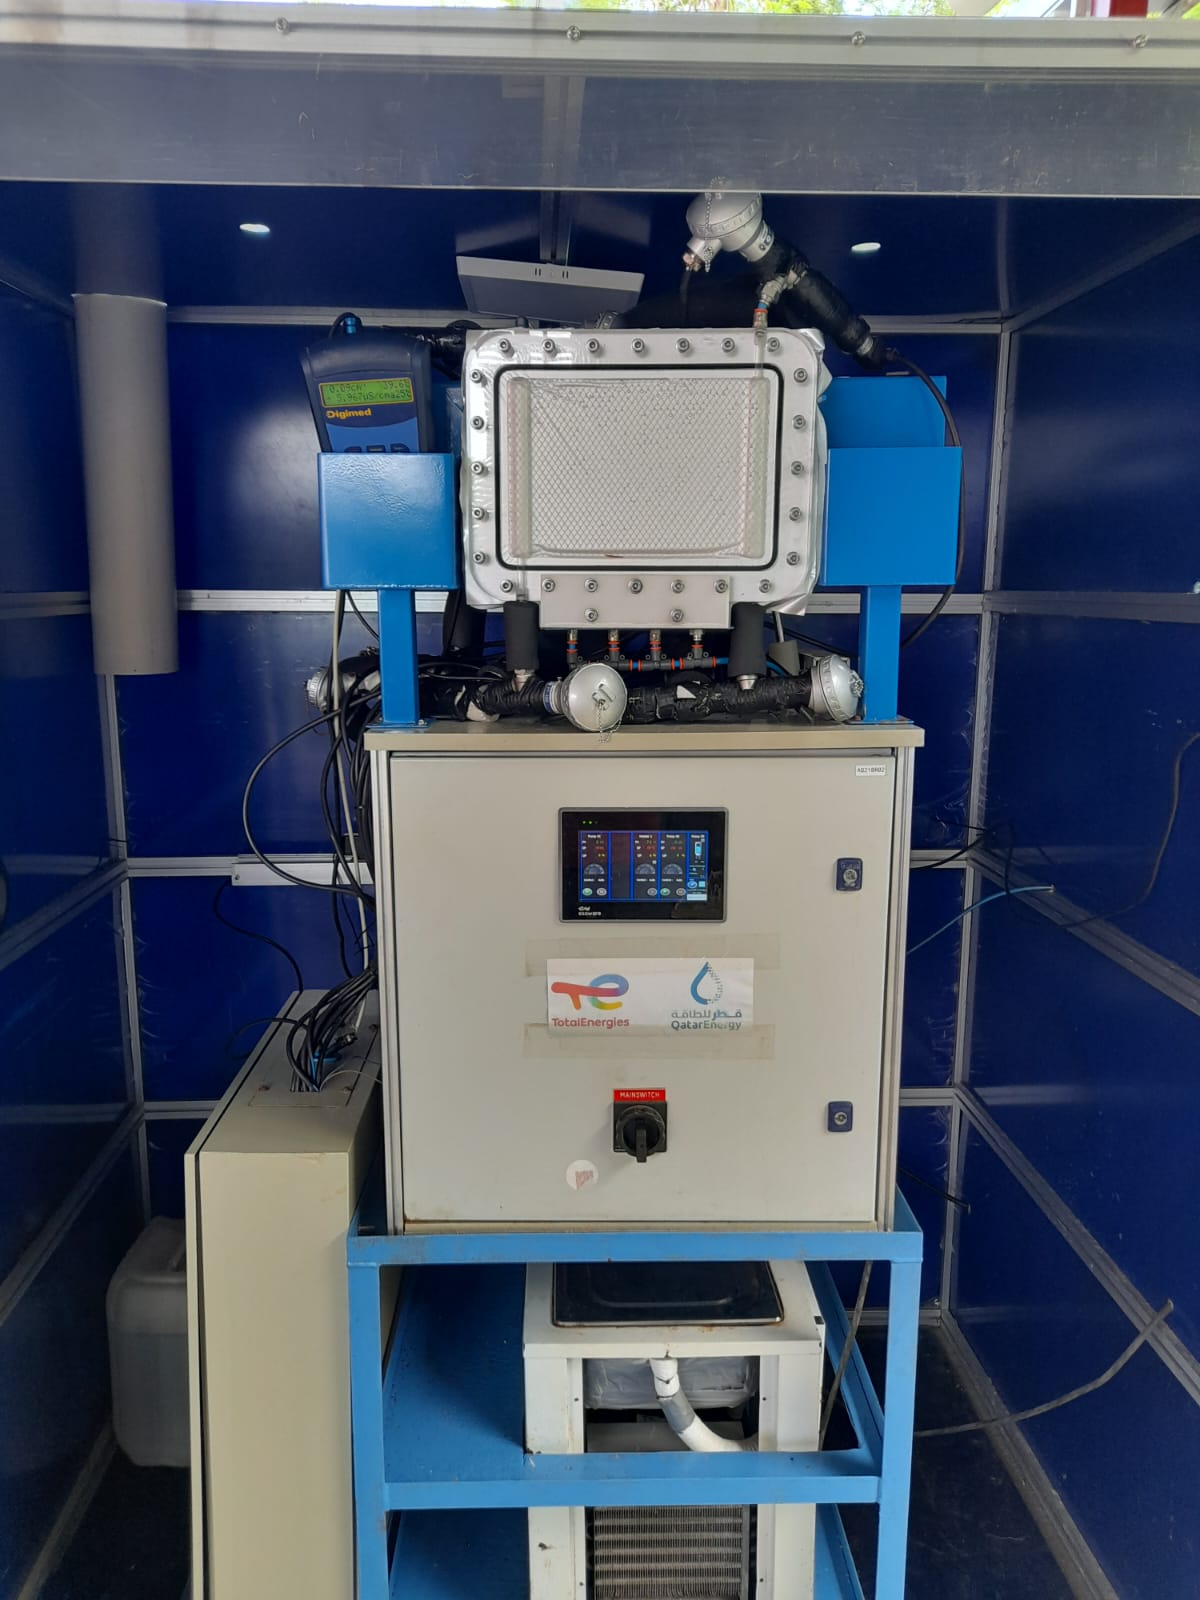
\includegraphics[width=\textwidth, height=9cm, keepaspectratio]{bancada.jpeg}
    \caption{Bancada utilizada para a realização dos experimentos.}
    \label{fig:bancada}
\end{figure}

A bancada também possui três bombas, uma para cada reservatório, as quais fornecem a alimentação do módulo AGMD, e uma para retornar o permeado produzido de volta ao reservatório de água de produção. A bancada é equipada com sensores de temperatura e pressão nas entradas e saídas do módulo, assim como sensores de vazão após as bombas dos reservatórios quente e frio. Há também uma célula de condutividade posicionada na linha de entrada do tanque de permeado. A tabela \ref{tab:sensores} apresenta as caracteristicas dos sensores utilizados e a figura \ref{fig:diagramabancada} o diagrama da bancada.

\begin{table}[H]
\centering
\caption{Sensores utilizados na bancada experimental.}
\label{tab:sensores}
\resizebox{\textwidth}{!}{%
\begin{tabular}{lllll}
\hline
\textbf{Sensor} & \textbf{Variável} & \textbf{Fabricante} & \textbf{Intervalo} & \textbf{Incerteza} \\ \hline
PT100 & Temperatura & Omega \cite{Omega} & 0--100~$^\circ$C & $\pm0.5~^\circ$C \\
Condutivímetro & Condutividade & Digimed \cite{Digimed} & 0--500~$mScm^{-1}$ & $\pm1\%$ da leitura \\
Transmissor de pressão & Pressão & Burkert \cite{Burkert1} & 0--10~bar & $\pm0,5\%$ FS \\
Medidor de vazão & Vazão & Burkert \cite{Burkert2} & 0,1--10~$Lmin^{-1}$ & $\pm1,5\%$ da leitura \\
\hline
\end{tabular}%
}
\end{table}

\begin{figure}[H]
    \centering
    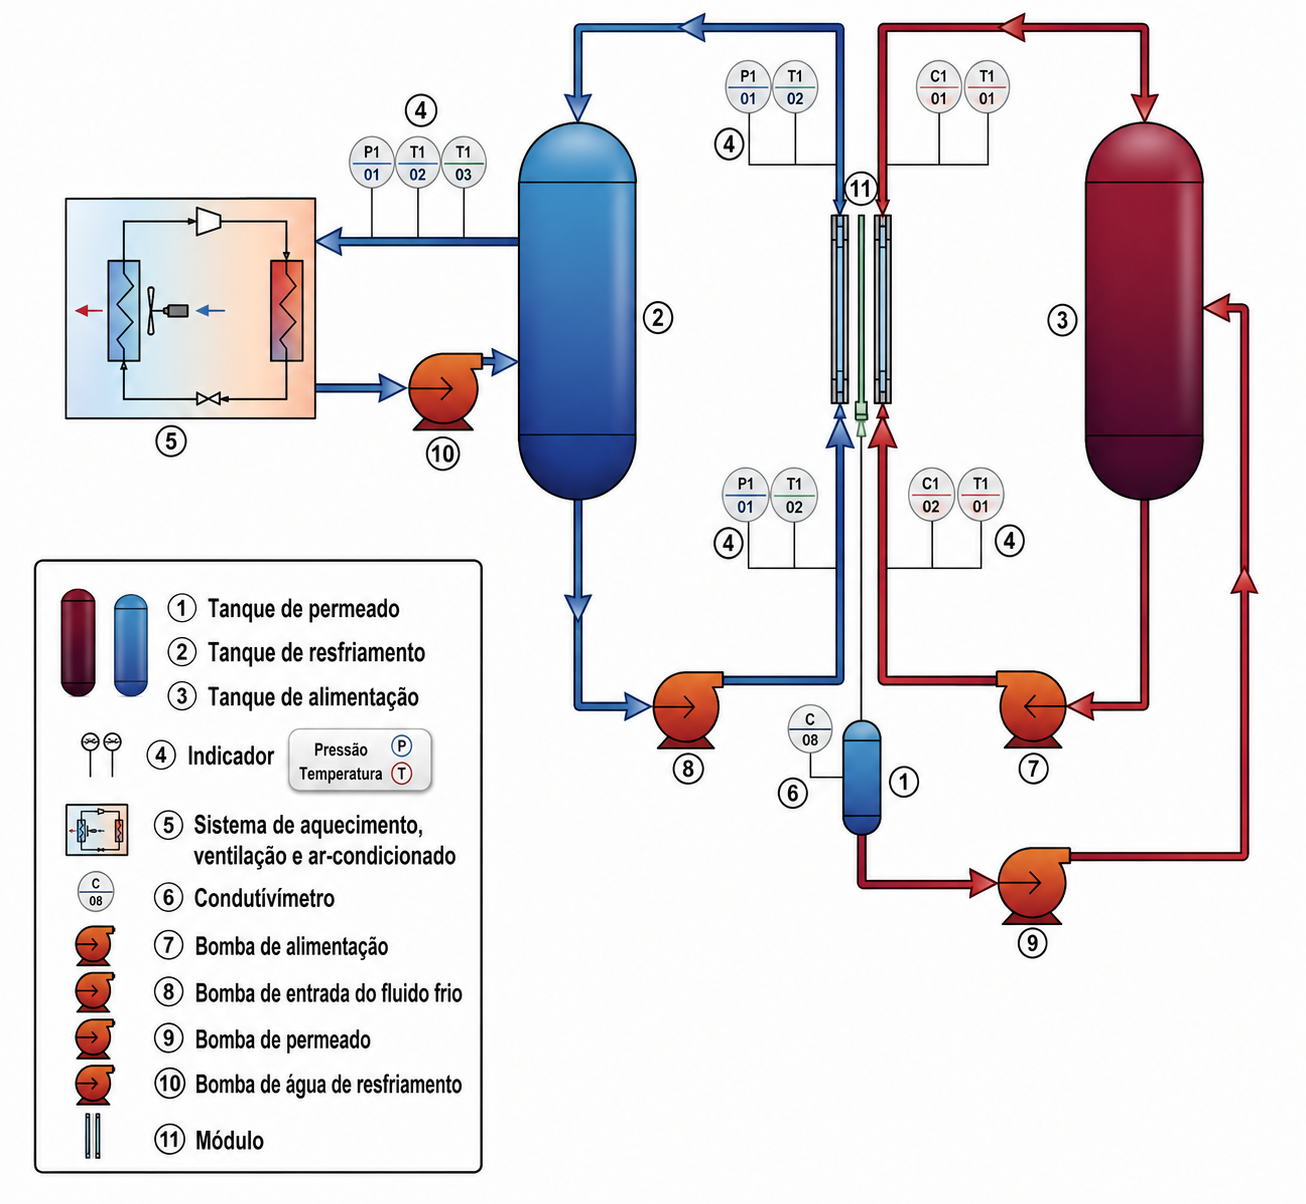
\includegraphics[width=\textwidth, height=12cm, keepaspectratio]{diagramabancada.png}
    \caption{Diagrama da bancada experimental de destilação por membranas com gap de ar (AGMD), contendo os tanques de alimentação, resfriamento e permeado, módulo de membrana, sistema HVAC, bombas de circulação e instrumentos de monitoramento de pressão, temperatura e condutividade.}
    \label{fig:diagramabancada}
\end{figure}

Os principais componentes do módulo AGMD são duas faces externas fabricadas em acrílico, uma folha de alumínio, um espaçador e a membrana a ser testada, a figura \ref{fig:vistaexplodida} apresenta uma vista expodida com estes componentes, enquanto a figura \ref{fig:modulomontado} apresenta o módulo montado.



\begin{figure}[H]
    \centering
    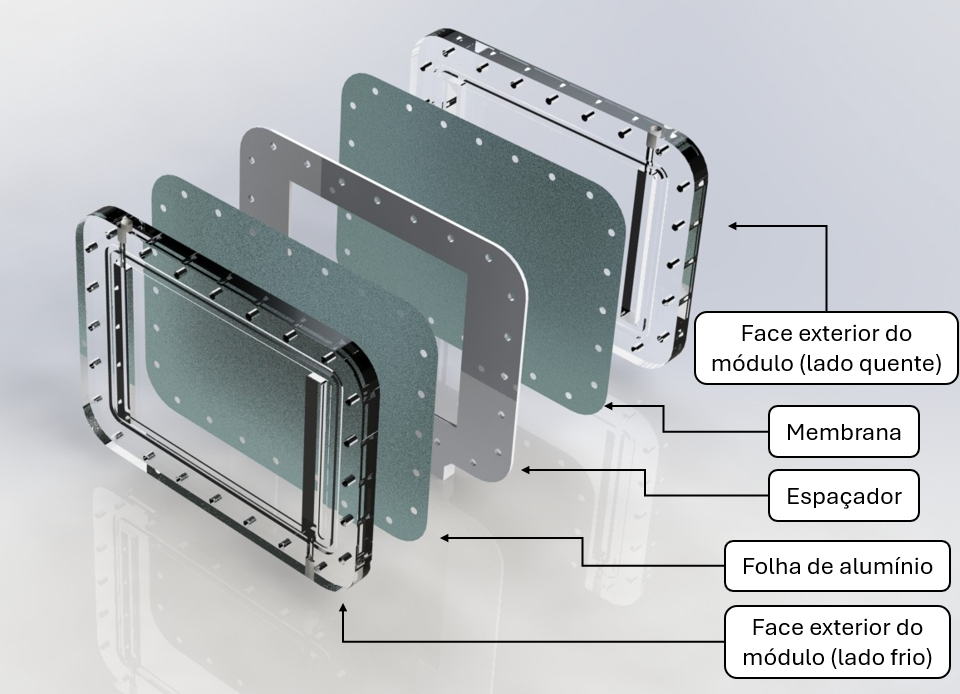
\includegraphics[width=\textwidth, height=7cm, keepaspectratio]{vistaexplodida.png}
    \caption{Vista explodida do módulo AGMD representado seus principais componentes.}
    \label{fig:vistaexplodida}
\end{figure}

\begin{figure}[H]
    \centering
    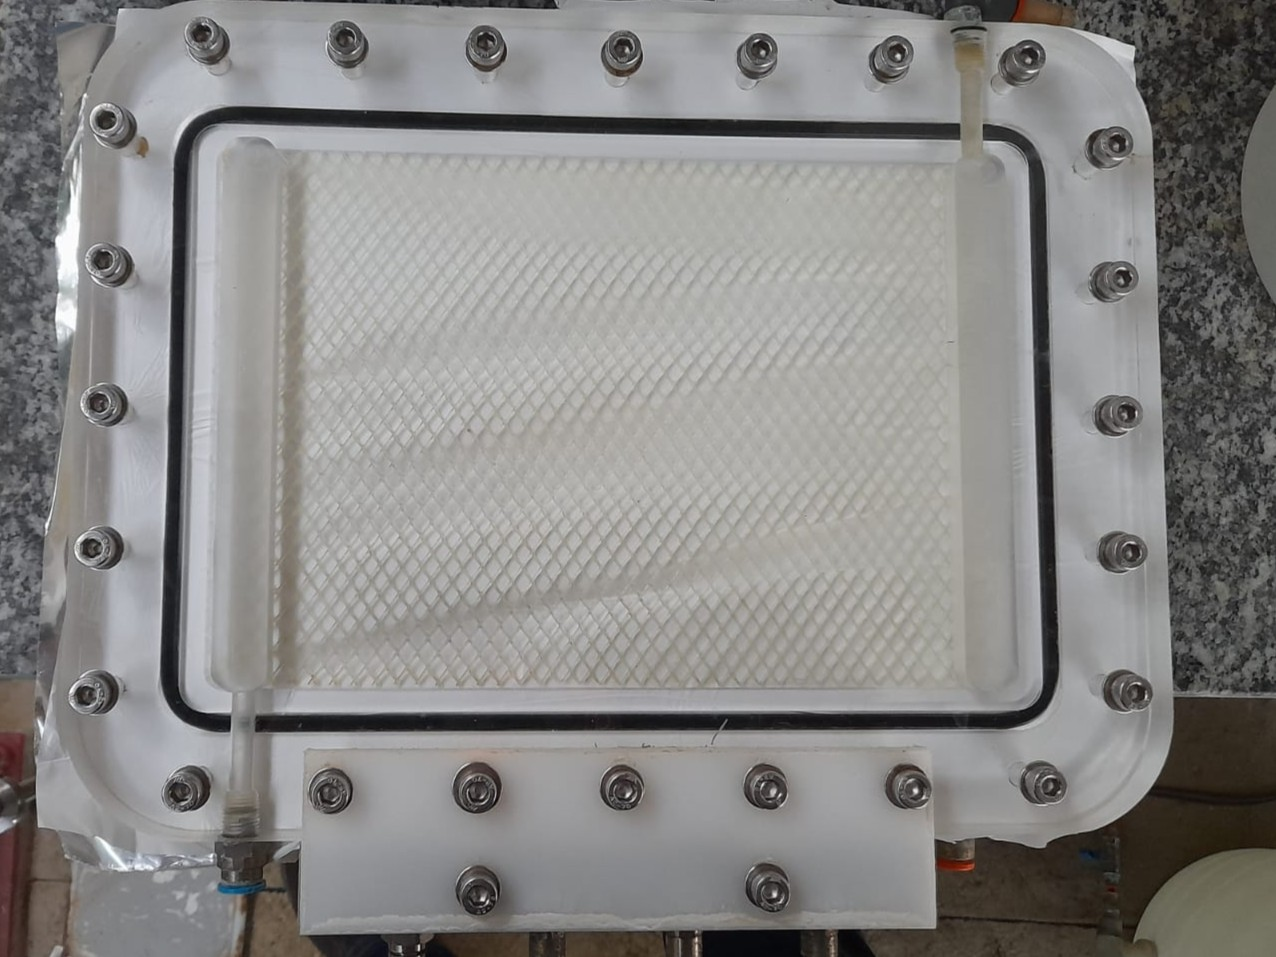
\includegraphics[width=\textwidth, height=7cm, keepaspectratio]{modulomontado.jpeg}
    \caption{Módulo montado em bancada.}
    \label{fig:modulomontado}
\end{figure}

Os experimentos serão realizados adotando a temperatura do lado quente em 70~$^\circ$C e do lado frio em 25~$^\circ$C, com vazão de 150~$Lh^{-1}$ em ambos os escoamentos. As membranas a serem avaliadas foram adquiridas do fabricante Tish \cite{TischScientific} e são fabricadas em diferentes materiais e suportes, descritos na tabela \ref{tab:membranas}.

\begin{table}[H]
\centering
\caption{Características das membranas utilizadas nos experimentos.}
\label{tab:membranas}

\begin{tabular}{lll}
\hline
\textbf{Amostra} & \textbf{Material da membrana} & \textbf{Suporte} \\ \hline

M1 & politetrafluoretileno expandido (ePTFE) & Polipropileno (PP) -- NET \\

M2 & politetrafluoretileno expandido (ePTFE) & Polipropileno (PP) \\

M3 & Polietileno (PE) & Sem suporte \\

M4 & Éster misto de celulose (MCE) & Sem suporte \\

M5 & politetrafluoretileno (PTFE) & Polipropileno (PP) \\

M6 & Polipropileno (PP) & Sem suporte \\

M7 & politetrafluoretileno (PTFE) & Polipropileno (PP) \\

M8 & politetrafluoretileno (PTFE) & Polipropileno (PP) \\

\hline
\end{tabular}
\end{table}


\section{Caracterização das membranas} 

Utilizou-se três equipamentos para o processo de caracterização das membranas: um porosimetro de fluxo capilar, Porolux, um microscópio digital, Hirox, e um goniômetro de ângulo de contato, Krüss. As análises de porosimetria e microscopia foram realizadas no LabMEMS, enquanto a medição de ângulo de contato foi realizada no LRAP.

A análise com o Porolux tem como objetivo determinar a distribuição de poros e a porosidade da membrana. Este ensaio tem início com a preparação da amostra da membrana a ser análisada. Tal preparação consiste em recortar um circúlo da membrana de acordo com o formato do suporte utilizado, com 25~mm de diâmetro no caso deste trabalho, e posteriormente encharcar a amostra com líquido de molhamento. 

Uma vez que as membranas utilizadas no estudo são hidrofóbicas, é necessário utilizar um líquido com baixa tensão superficial. Deste modo, utilizou-se como líquido de molhamento o Porefil (tensão superficial de 16,07 $\pm$ 0,05 $mNm^{-1}$), comercializado pela mesma fabricante do porosimetro, a Porometer. Para garantir o completo molhamento da amostra, a mesma foi submersa por um minuto no Porefil.

Posteriormente a preparação, a amostra é posicionada no suporte e inicia-se o experimento, o qual consiste na aplicação de nitrogênio pressurizado na face hidrofóbica da membrana, de modo gradual, até que seja observada uma pequena queda de pressão, indicando a abertura do poro com maior diâmetro (bubble point), como estabelecido pela norma ASTM F316-3~\cite{ASTM_F316_03}. 

Após a determinaçao do bubble point, o equipamento segue aumentando a pressão aplicada sobre a membrana até alcançar a pressão estabelecida pelo usuário. Estabelece-se a pressão final do experimento em função da curva molhada obtida ao longo do experimento, de modo que a pressão definida é aquela em que a curva se torna linear, momento onde todos os poros da membrana estão abertos.  

Para a determinação da curva seca da membrana, utilizou-se o método de cálculo disponível no software do equipamento. A figura \ref{fig:exemplocurvas} ilustra as curvas geradas pelo equipamento ao final dos ensaios. Repetiu-se este procedimento para três amostras de cada membrana. Como resultado, obteve-se a distribuição de poros, o diâmetro médio e a porosidade das membranas estudadas.

\begin{figure}[H]
    \centering
    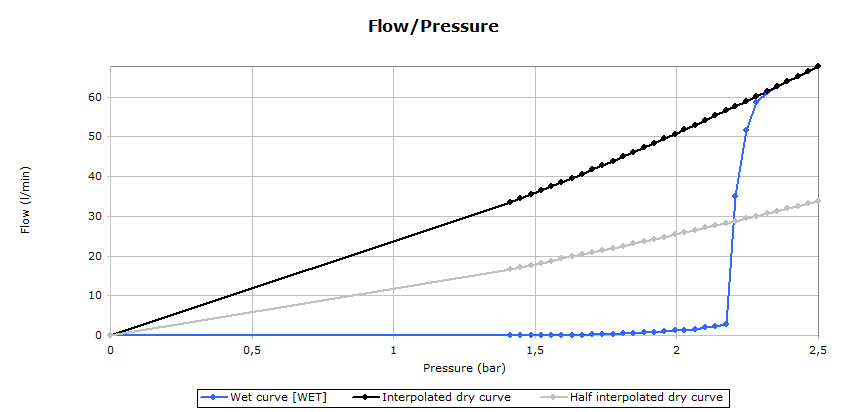
\includegraphics[width=\textwidth, height=6cm, keepaspectratio]{exemplocurvasporometer.png}
    \caption{Exemplo das curvas seca e molhada gerada pelo Porometer.}
    \label{fig:exemplocurvas}
\end{figure}


A análise com o goniômetro utiliza o método da séssil, onde uma gota de água deionizada é colocada sobre a superfície da membrana e fotografado por um sistema de alta resolução, permitindo medir o ângulo de contato entre a superfície da membrana e a gota. Foram realizadas três medições para cada membrana. A análise com o microcópio digital permitiu visualizar a estrutura dos suportes empregados nas membranas. A figura \ref{fig:hirox} apresenta os equipamentos utilizados.

 \begin{figure}[H]
    \centering
    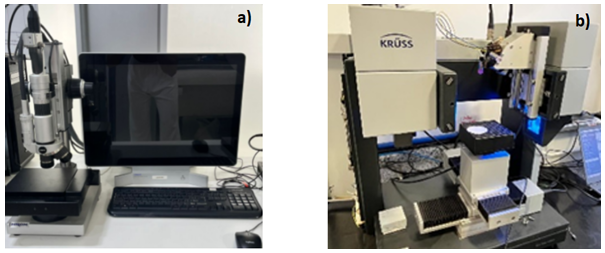
\includegraphics[width=\textwidth, height=12cm, keepaspectratio]{hirox.png}
    \caption{Microscópio digital a) e goniômetro de ângulo de contato b) utilizados no processo de caracterização das membranas.}
    \label{fig:hirox}
\end{figure}

\section{Características da água de produção}

A água de produção utilizada nos experimentos pertence a um campo de extração localizado no Brasil. A composição da água de produção foi definida através de duas amostras, retiradas em dias distintos. A análise da composição da água foi realizada pela empresa que forneceu as amostras.

Uma vez que os compostos orgânicos apresentam alta volatilidade em temperatura ambiente, adicionou-se a concentração dos mesmos à água de produção, em via de garantir a presença destes contaminantes.

\begin{table}[H]
\centering
\caption{Características analíticas de referência da água de produção utilizada nos experimentos.}
\label{tab:produced_water}

\begin{tabular}{lccc}
\hline
\textbf{Parâmetro} & \textbf{Unidade} & \textbf{18/Jan/2024} & \textbf{10/Jul/2024} \\ \hline

\multicolumn{4}{l}{\textbf{Análises físico-químicas}} \\

pH (25~$^\circ$C) & -- & 6,18 & 6,56 \\
Temperatura & $^\circ$C & 24,80 & 25,00 \\
Nitrogênio amoniacal & $mgL^{-1}$ & 36,00 & 81,00 \\
Óleos e graxas & $mgL^{-1}$ & $<$5,00 & $<$5,00 \\
Carbono orgânico total (COT) & $mgL^{-1}$ & 597,20 & 0,60 \\
Salinidade & \% & 23,50 & 23,50 \\

\hline

\multicolumn{4}{l}{\textbf{Metais}} \\

Bário & $mgL^{-1}$ & 9,62 & 14,50 \\
Ferro & $mgL^{-1}$ & 0,23 & 0,67 \\
Manganês & $mgL^{-1}$ & 0,13 & 0,14 \\
Zinco & $mgL^{-1}$ & $<$0,05 & 0,14 \\

\hline

\multicolumn{4}{l}{\textbf{Compostos orgânicos BTEX}} \\

Benzeno & $\mu gL^{-1}$ & 5523,11 & 2203,33 \\
Tolueno & $\mu gL^{-1}$ & 4055,78 & 1918,89 \\
Etilbenzeno & $\mu gL^{-1}$ & 471,78 & 177,06 \\
Xilenos totais & $\mu gL^{-1}$ & 2727,11 & 1096,00 \\

\hline

\multicolumn{4}{l}{\textbf{Hidrocarbonetos aromáticos policíclicos (PAHs)}} \\

Fenantreno & $\mu gL^{-1}$ & 6,34 & 1,53 \\
Fluoreno & $\mu gL^{-1}$ & 1,65 & 0,49 \\
Naftaleno & $\mu gL^{-1}$ & 84,27 & 1,34 \\

\hline
\end{tabular}
\end{table}
\newpage

\section{Análise de dados}

Calculou-se o LEP com base nos resultados obtidos durante a caracterização das membranas através da equação de Young-Laplace \ref{eq:LEP}:

\begin{equation}
    LEP = -\frac{2 \cdot B \cdot \gamma_L \cos\theta}{r_{\max}},
    \label{eq:LEP}
\end{equation}

onde $\gamma_L$ é a tensão superficial do líquido, $\theta$ é o ângulo de contato entre o líquido e a superfície da membrana, $r_{\max}$ é o maior raio de poro da membrana e $B$ o fator de forma atribuído ao poro. No presente estudo o fator de forma foi considerado como 1, de modo a considerar o poro como um cilindro ideal. 

Os parâmetros de performance do equipamento serão calculados em função da transferência de calor no lado quente e frio do módulo, além do fluxo de permeado produzido. A taxa de transferência de calor no lado quente e frio foram calculadas através das equações \ref{eq:Qcold} e \ref{eq:Qhot}, respectivamente: 

\begin{equation}
    Q_{\mathrm{cold}} = \dot{m}_c \, c_{p,c} \left( T_{c,out} - T_{c,in} \right),
    \label{eq:Qcold}
\end{equation}

\begin{equation}
    Q_{\mathrm{hot,sens}} = \dot{m}_h \, c_{p,h} \left( T_{h,in} - T_{h,out} \right),
    \label{eq:Qhot}
\end{equation}

onde $\dot m$ é a vazão mássica, $c_p$ é o calor específico, os subscritos $h, c, in, out$ representam o lado quente, frio, entrada e saída, respectivamente. As propiedades termofísicas da água de produção, como densidade e calor específico, serão avaliadas em função da salinidade através das correlações propostas por \cite{Millero1980}.

Uma estimativa da quantidade de calor fornecida pelo módulo para a evaporação do permeado será calculada através da equação \ref{eq:Qvap}, onde $T_{ref}$ é a temperatura de referência, calculada considerando as temperaturas dos escoamentos frio e quente através da equação \ref{eq:Tref}.

\begin{equation}
    Q_{\mathrm{vap}} = \dot{m}_p \, h_{lv}(T_{\mathrm{ref}}),
    \label{eq:Qvap}
\end{equation}

\begin{equation}
    T_{\mathrm{ref}} =
\frac{
\left( T_{h,in} + T_{h,out} \right)/2
+
\left( T_{c,in} + T_{c,out} \right)/2
}{2}
    \label{eq:Tref}
\end{equation}

O fluxo de permeado será obtido através de um sensor de pressão instalado no fundo do reservatório de permeado, obtido através da equação \ref{eq:fluxo}, onde $A_B$ é a área da base do reservatório de permeado, $A_m$ é a área efetiva da membrana, g é a gravidade, $\Delta P / \Delta t$ é a taxa de variação da pressão ao longo do tempo, obtendo-se o resultado em $kgm^{-2}h^{-1}$.

\begin{equation}
J = \frac{A_B}{g \, A_m}
\left( \frac{\Delta P}{\Delta t} \right)
3600
    \label{eq:fluxo}
\end{equation}

O índice de rejeição instantânea de íons, IJR, será obtido através da equação \ref{eq:IJR}, onde $k_p$ e $k_f$ representam as condutividades do permeado e da água de produção, respectivamente. 

\begin{equation}
IJR =
\left(
1 - \frac{\kappa_p}{\kappa_f}
\right)
\times 100
    \label{eq:IJR}
\end{equation}

O fator de desempenho térmico, GOR, será calculado através da equação \ref{eq:GOR} como a razão entre o calor latente associado ao fluxo de permeado pelo calor sensível fornecido ao módulo.

\begin{equation}
GOR = \frac{\dot{m}_p \, h_{lv}}{Q_{\mathrm{hot}}}
    \label{eq:GOR}
\end{equation}

Por fim, o consumo de energia térmica específica será calculada através da equação \ref{eq:SEC}, como a razão entre a energia térmica fornecida pelo volume de permeado produzido, $V_p$.

\begin{equation}
SEC_{\mathrm{th}} =
\frac{Q_{\mathrm{hot}}}{V_p}
\quad
\left[\mathrm{J/m^3}\right]
    \label{eq:SEC}
\end{equation}

As incertezas associadas as variáveis primárias de medição, como temperatura, vazão, pressão e condutividade serão propagadas através aos indicadores de performance através da lei de propagação de variáveis.
  \chapter{Resultados Preliminares}

\section{Caracterização das membranas}

O processo de caracterização das membranas gerou como resultado as informações sobre diâmetro de poro médio, diâmetro máximo, ângulo de contato e LEP. Dentre as membranas testadas, as membranas M4 e M6 apresentaram diâmetros de poro médio com aproximadamente uma ordem de grandeza superior as demais. A incerteza associada aos diâmetros de poro foi calculada considerando que os dados possuem uma distribuição normal. Uma análise estatistica mais aprofundada será realizada posteriormente para uma análise de incerteza mais acertiva. A figura \ref{fig:diamporo} apresenta os diâmetros de poro médio das membranas estudadas. As figuras \ref{fig:distporo1} e \ref{fig:distporo2} apresentam as distribuições de poro obtidas.

\begin{figure}[H]
    \centering
    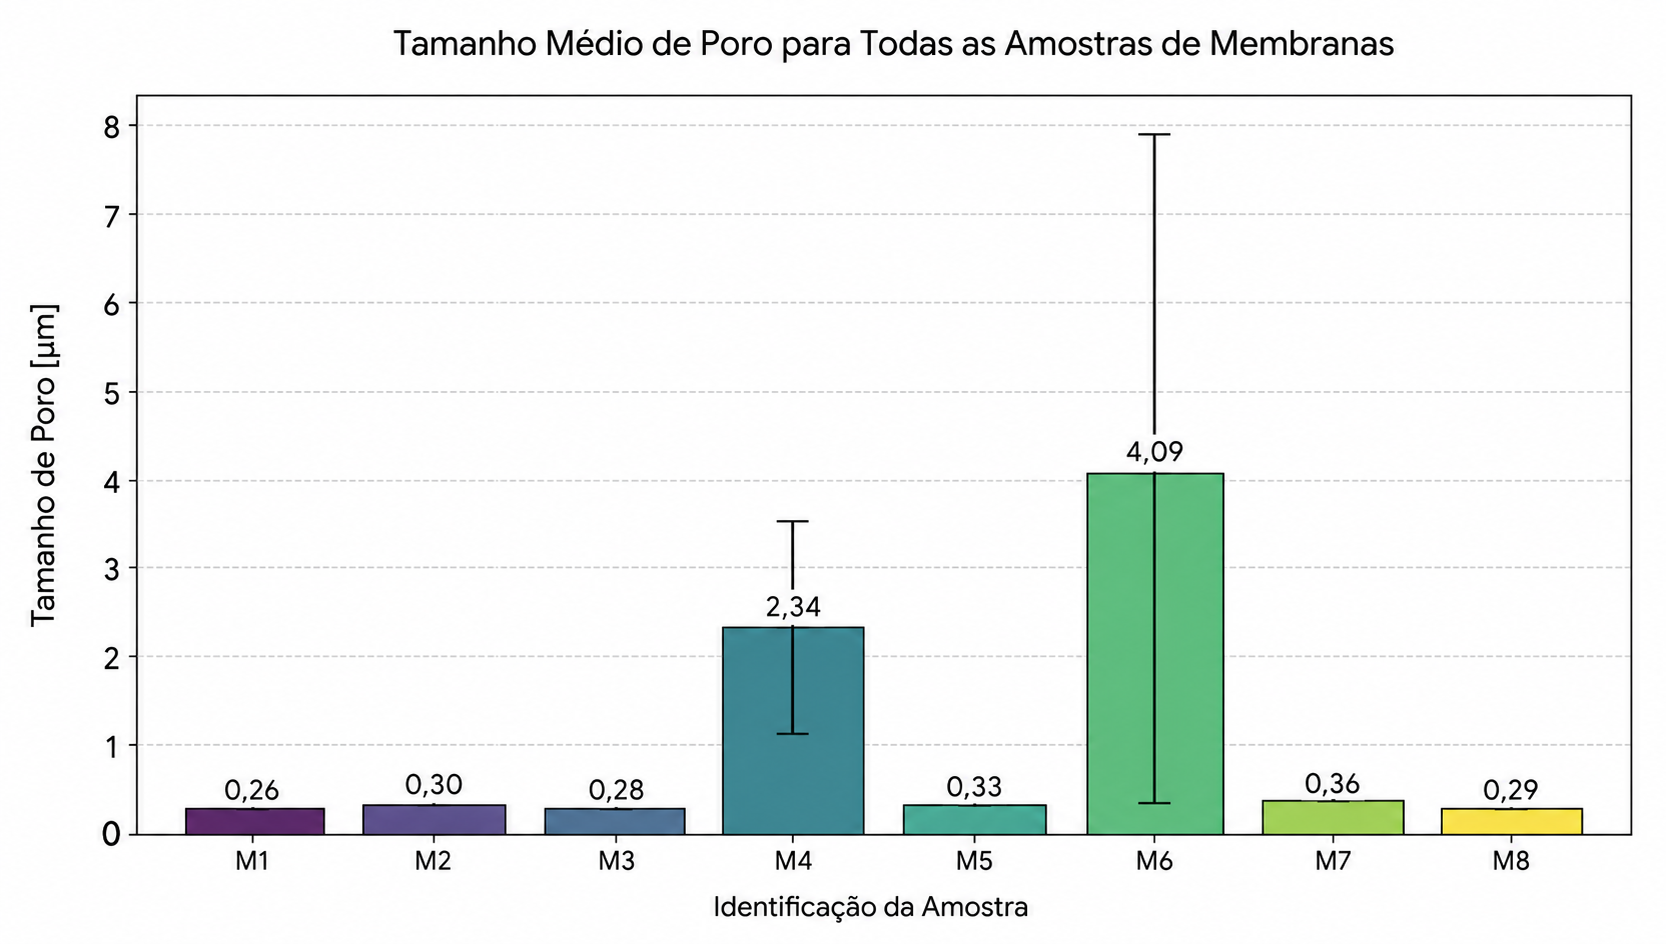
\includegraphics[width=\textwidth, height=8cm, keepaspectratio]{diametrodeporo.png}
    \caption{Diâmetro de poro médio das membranas analisadas, obtidos através de porosimetria de fluxo capilar.}
    \label{fig:diamporo}
\end{figure}

\begin{figure}[H]
    \centering
    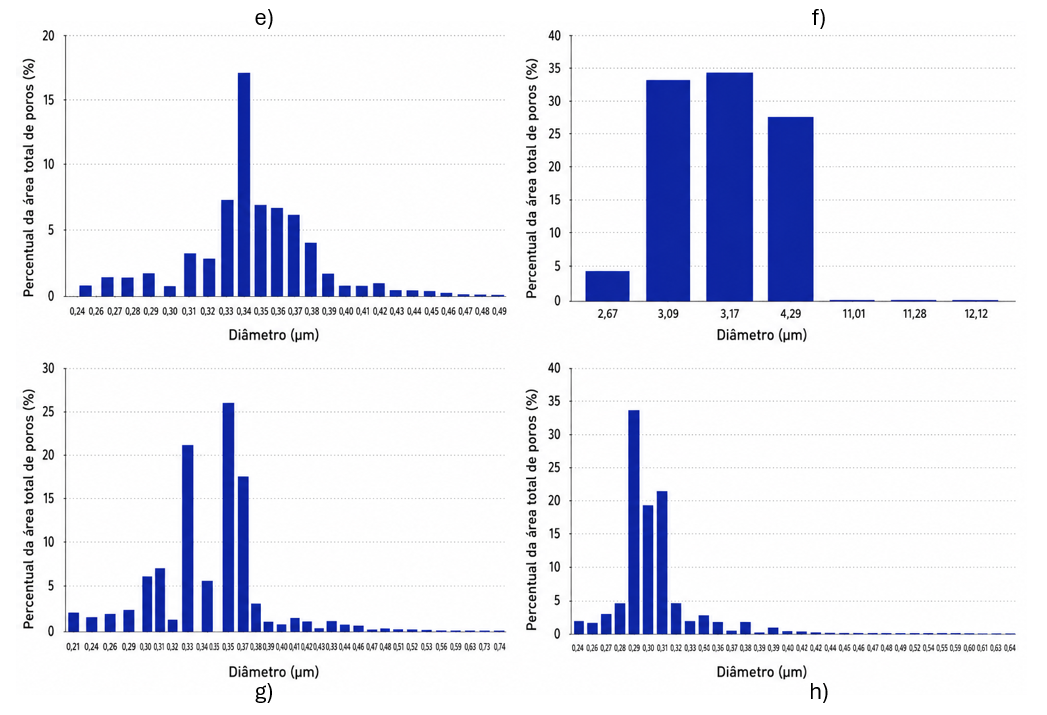
\includegraphics[width=\textwidth, height=12cm, keepaspectratio]{distporom5m8.png}
    \caption{Distribuições do diâmetro de poros obtidas para as membranas M1 a), M2 b), M3 c) e M4 d). }
    \label{fig:distporo1}
\end{figure}

\begin{figure}[H]
    \centering
    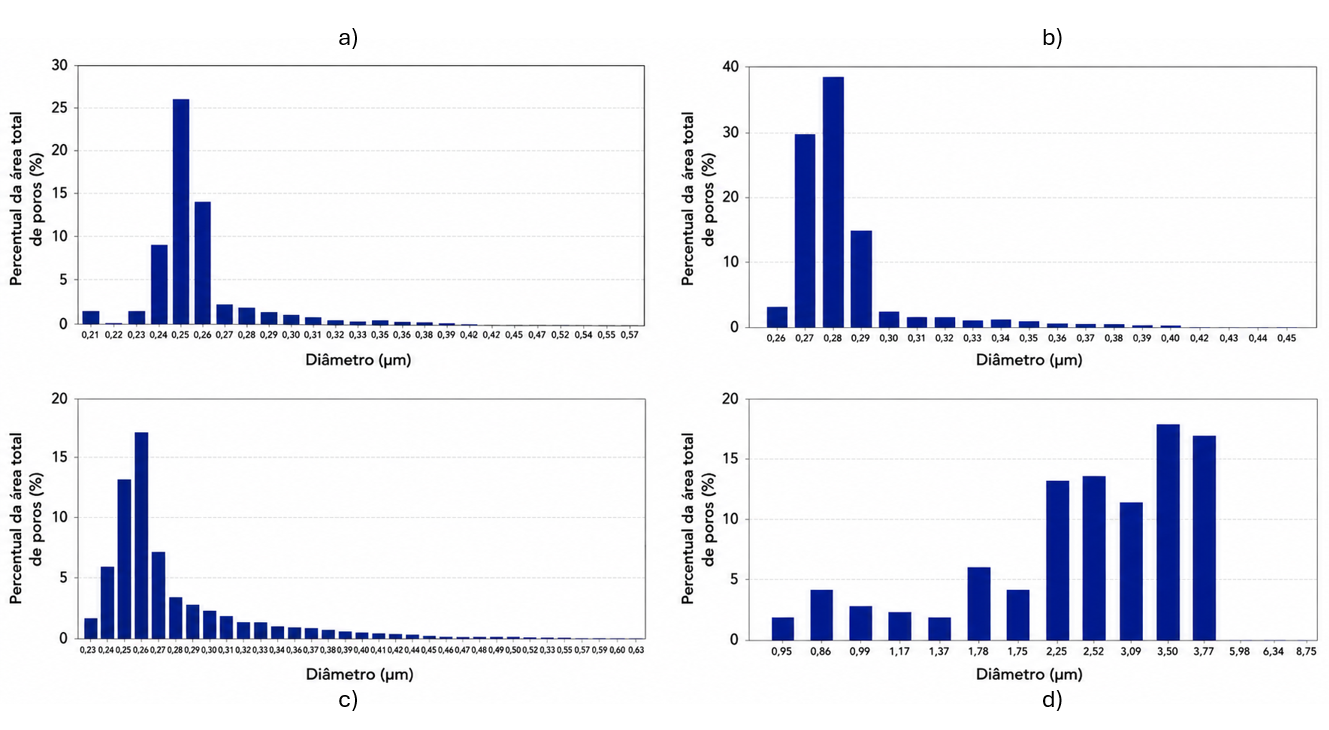
\includegraphics[width=\textwidth, height=12cm, keepaspectratio]{distporom1m4.png}
    \caption{Distribuições do diâmetro de poros obtidas para as membranas M5 a), M6 b), M7 c) e M8 d). }
    \label{fig:distporo2}
\end{figure}

As medições de ângulo de contato indicaram que as membranas encontram-se dentro da faixa hidrofóbica requerida para o processo de destilação por membranas. A figura \ref{fig:angulodecontato} apresentam as medições de ângulo de contato realizadas.

\begin{figure}[H]
    \centering
    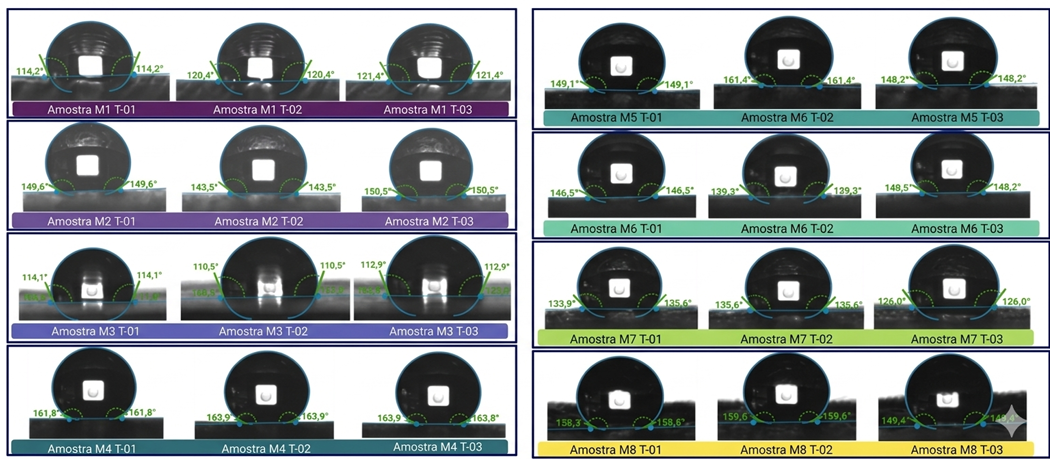
\includegraphics[width=\textwidth, height=12cm, keepaspectratio]{angulodecontato.png}
    \caption{Medições de ângulo de contato das membranas estudadas.}
    \label{fig:angulodecontato}
\end{figure}

Com base nos resultados obtidos nas análises de porosimetria e ângulo de contato, calculou-se o LEP utilizando a equação \ref{eq:LEP}.

\begin{figure}[H]
    \centering
    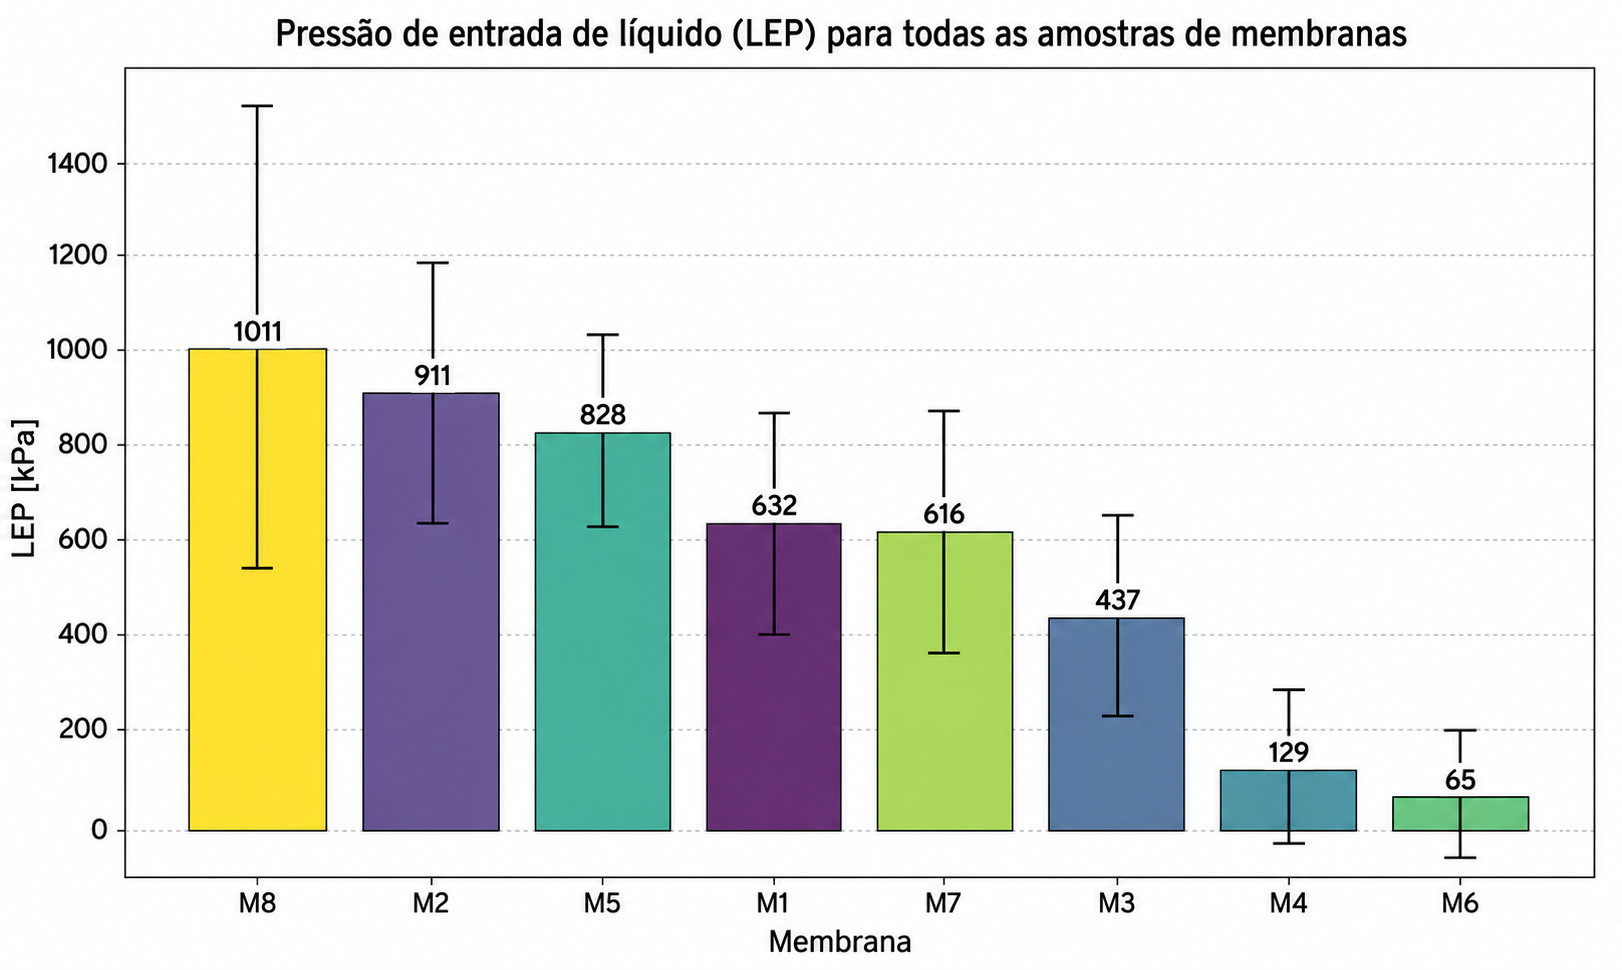
\includegraphics[width=\textwidth, height=12cm, keepaspectratio]{LEP.png}
    \caption{LEP calculado para as membranas estudadas.}
    \label{fig:angulodecontato}
\end{figure}
  \chapter{Considerações finais}

A presente dissertação tem como objetivo avaliar o desempenho de longo prazo de membranas comerciais no tratamento de água de produção via destilação por membranas. As análises serão realizadas em oito membranas com diferentes características morfológicas, incluindo material, suporte, diâmetro de poro e ângulo de contato.Os experimentos serão conduzidos em uma bancada equipada com um módulo AGMD, utilizando água de produção como corrente de alimentação, conforme as condições operacionais descritas no Capítulo 3. 

Os resultados obtidos serão comparados com o propósito de investigar a influência das diferentes características morfológicas das membranas sobre o desempenho do processo de tratamento da água de produção, considerando parâmetros como fluxo de permeado, estabilidade operacional e resistência ao molhamento.

Os resultados preliminares apresentados no Capítulo 4 evidenciam as principais características morfológicas das membranas avaliadas, incluindo diâmetro médio de poro , distribuição de poro, ângulo de contato e LEP. De modo geral, os resultados indicam que as membranas possuem potencial para aplicação em processos de destilação por membranas, em função de suas características hidrofóbicas. 

Em relação ao LEP, as membranas M4 e M6 apresentam maior probabilidade de molhamento, associada aos elevados diâmetros de poro observados. Além disso, verificou-se que as distribuições de poro das membranas diferem significativamente de uma distribuição normal. Dessa forma, será realizada uma análise estatística mais aprofundada, com o objetivo de determinar as incertezas associadas aos parâmetros avaliados de maneira mais representativa e confiável.

Por fim, ressalta-se que os materiais e equipamentos necessários para a conclusão da pesquisa encontram-se disponíveis no LabMEMS e em laboratórios parceiros. O cronograma para a realização da pesquisa é apresentado na figura \ref{fig:cronograma}.

\begin{figure}[H]
    \centering
    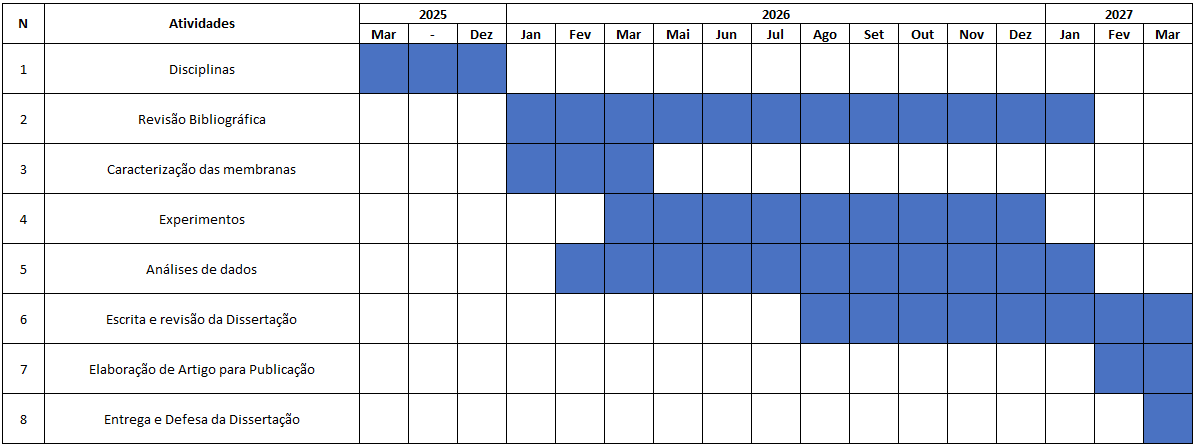
\includegraphics[angle=90, width=\textwidth, height=20cm, keepaspectratio]{cronograma.png}
    \caption{Cronograma da dissertação.}
    \label{fig:cronograma}
\end{figure}
  
 \backmatter

  \makeatletter
  \renewenvironment{thebibliography}[1]
     {\chapter*{\bibname}
      \list{\@biblabel{\@arabic\c@enumiv}}
           {
            \settowidth\labelwidth{\@biblabel{#1}}
            \leftmargin=\labelwidth
            \advance\leftmargin\labelsep
            \itemindent=0pt
            \listparindent=0pt
            \parsep=0pt
            \itemsep=0.2cm
            \usecounter{enumiv}
            \let\p@enumiv\@empty
            \renewcommand\theenumiv{\@arabic\c@enumiv}
           }
      \sloppy}
     {\endlist}
  \makeatother

  \bibliographystyle{coppe-unsrt}
  \bibliography{Bibliography/references}

  \appendix
\end{document}
%% 
%%
%% End of file `example.tex'.